\documentclass[11pt]{book}

\usepackage{longtable}
\usepackage{xcolor}
\usepackage{fontspec}
\setmainfont[
Path = fonts/, 
UprightFont = TitilliumWeb-Regular.ttf,
BoldFont = TitilliumWeb-Bold.ttf,
ItalicFont = TitilliumWeb-Italic.ttf,
BoldItalicFont = TitilliumWeb-BoldItalic.ttf
]{TitilliumWeb}

%\usepackage[utf8]{inputenc}
%\usepackage{listingsutf8}
%\lstset{inputencoding=utf8}

\usepackage{tikz}
\usetikzlibrary{arrows.meta, positioning}


\usepackage{tabularx}
\usepackage[a4paper,outer=3cm,inner=3cm,top=3cm,bottom=3cm]{geometry}
\usepackage[colorlinks=true, linkcolor=black, citecolor=blue, urlcolor=blue]{hyperref}
\usepackage{graphicx}
\usepackage{xcolor}
\graphicspath{{images/}}
\usepackage{svg}


\usepackage{listings}
\lstdefinestyle{SqlStyle}{
	language=SQL,
	basicstyle=\ttfamily\footnotesize,
	morekeywords={REAL, TEXT, REFERENCES},
	keywordstyle=\color{blue},
	commentstyle=\color{gray},
	stringstyle=\color{red},
	breaklines=true,
	showstringspaces=false,
	tabsize=2,
	captionpos=b,
	numbers=left,
	numberstyle=\tiny\color{gray},
	frame=lines,
	backgroundcolor=\color{lightgray!10},
	comment=[l]{//},
	morecomment=[s]{/*}{*/},
	commentstyle=\color{gray}\ttfamily,
	string=[s]{'}{'},
	morestring=[s]{"}{"},
	%	stringstyle=\color{teal}\ttfamily,
	%	showstringspaces=false
}

\lstdefinelanguage{bash} {
	keywords={},
	basicstyle=\ttfamily\small,
	keywordstyle=\color{blue}\bfseries,
	ndkeywords={iex},
	ndkeywordstyle=\color{purple}\bfseries,
	sensitive=true,
	commentstyle=\color{gray},
	stringstyle=\color{red},
	numbers=left,
	numberstyle=\tiny\color{gray},
	breaklines=true,
	frame=lines,
	backgroundcolor=\color{lightgray!10},
	tabsize=2,
	comment=[l]{\#},
	morecomment=[s]{/*}{*/},
	commentstyle=\color{gray}\ttfamily,
	stringstyle=\color{purple}\ttfamily,
	showstringspaces=false
}

\usepackage{plantuml}
\usepackage{tikz}
\usetikzlibrary{shapes.geometric, arrows.meta, positioning}

\newcommand{\authors}[1]{{\chapterauthor{#1}\addtocontents{toc}{#1\par}}}
\newcommand{\HUGE}{\fontsize{40}{48}\selectfont}

\renewcommand{\contentsname}{Daftar Isi}
\renewcommand{\chaptername}{Bab}
\renewcommand{\figurename}{Gambar}

\makeatletter
\newcommand{\chapterauthor}[1]{%
	{\parindent0pt\vspace*{-25pt}%
		\linespread{1.1}\large\scshape#1%
		\par\nobreak\vspace*{35pt}}
	\@afterheading%
}
\makeatother

\begin{document}


\begin{titlepage}
	\begin{tikzpicture}[remember picture, overlay]
		% Gambar latar belakang atau logo
		\node[anchor=north west, inner sep=0pt] at ([xshift=.18\textwidth, yshift=-.1\textwidth] current page.north west){
			
\includegraphics[width=.3\paperwidth]{../figures/logo_universitas.png} 
		};
	
		\node[anchor=north west, inner sep=0pt, opacity=.12] at (current page.north west){
			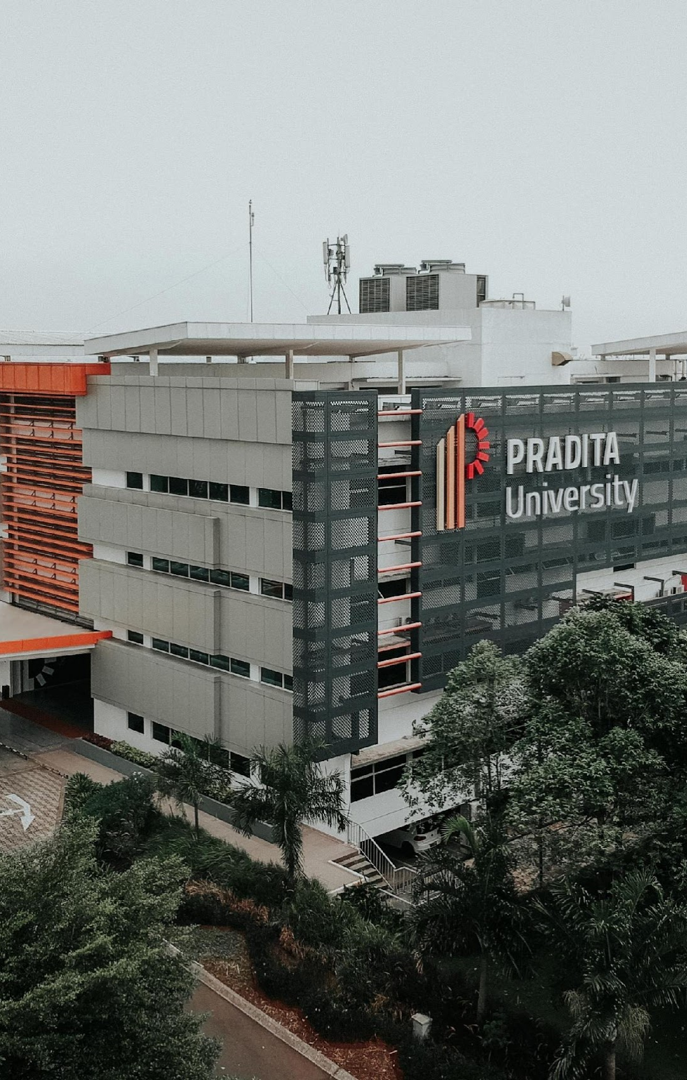
\includegraphics[width=\paperwidth]{../figures/building.png}
		};
		
		% Judul Tengah
		\node[anchor=center] at ([yshift=.1\textheight]current page.center) {
			\begin{minipage}{\textwidth}
				
				{\LARGE \textbf{Course Module -- IT140704}}\\[0.03\textheight] % Book Type
				{\HUGE \textcolor{orange}{\textbf{Big Data for Business}}}\\[.04\textheight] % Title
%				{\Huge \textcolor{orange}{\textbf{Penggunaan Large-language Model}}}\\[.08\textheight] % Subtitle
				{\LARGE \textbf{Alfa Yohannis}}\\[0.05\textheight] % Authors
			\end{minipage}
		};
		
		% Teks bawah dengan latar oranye penuh dan teks putih
		\node[anchor=south west] at (
		current page.south west) {
			\begin{tikzpicture}[remember picture, overlay]
				\node[anchor=south west, fill=orange, text=white, minimum width=\paperwidth, minimum height=.14\textheight, align=center, font=\Huge\bfseries] at (-.15,-.15) {
					Master's in Information Technology\\
					Pradita University
				};
			\end{tikzpicture}
		};
	\end{tikzpicture}
\end{titlepage}
	
	% Contents Page
	\tableofcontents
	
	\chapter{Pendahuluan}

\section{Latar Belakang}

Di era transformasi digital saat ini, data telah menjadi aset strategis bagi organisasi di berbagai sektor. Volume data yang terus meningkat, baik dari transaksi internal, interaksi pelanggan, hingga media sosial, menciptakan peluang besar sekaligus tantangan dalam pengambilan keputusan yang efektif dan berbasis bukti. Istilah \textit{big data} mencerminkan kompleksitas data modern yang ditandai oleh karakteristik Volume, Variety, Velocity, Veracity, dan Value (5V).

Bagi kalangan manajerial dan pengambil kebijakan, pemahaman mengenai big data tidak lagi terbatas pada aspek teknis, melainkan lebih pada bagaimana data dapat dimanfaatkan untuk menciptakan nilai bisnis, meningkatkan efisiensi operasional, memahami perilaku konsumen, serta mendukung inovasi berbasis analitik.

\section{Tujuan Pembelajaran}

Mata kuliah ini bertujuan untuk membekali mahasiswa pascasarjana dari latar belakang manajemen dan bisnis dengan pemahaman konseptual dan keterampilan praktis dalam mengelola dan memanfaatkan big data. Tanpa memerlukan latar belakang pemrograman atau teknologi informasi, mahasiswa akan diperkenalkan pada teknologi big data, pendekatan analitik, serta kerangka pengambilan keputusan berbasis data.

Secara khusus, tujuan pembelajaran mencakup:

\begin{itemize}
	\item Memahami konsep, karakteristik, dan peran strategis big data dalam organisasi.
	\item Mampu menjelaskan infrastruktur dan arsitektur teknologi big data secara konseptual.
	\item Menggunakan alat bantu visual (Power BI, Orange, KNIME) untuk eksplorasi data, analisis prediktif, dan visualisasi.
	\item Menganalisis kasus penggunaan big data dalam berbagai sektor industri.
	\item Mengidentifikasi tantangan etika, tata kelola, dan monetisasi data dalam konteks organisasi.
\end{itemize}

\section{Ruang Lingkup Materi}

Materi dalam mata kuliah ini disusun secara bertahap, mencakup empat area pembelajaran utama:

\begin{enumerate}
	\item \textbf{Dasar-dasar dan Strategi Big Data:} pengenalan konsep big data, kerangka kerja strategis seperti \textit{Big Data Value Chain}, \textit{5Vs}, \textit{Big Data Maturity Model} (BDMM), dan arsitektur teknologi data.
	
	\item \textbf{Pengelolaan dan Pemrosesan Data:} mencakup pemahaman basis data (SQL dan NoSQL), proses pembersihan data, dan integrasi sumber data.
	
	\item \textbf{Analisis dan Pengambilan Keputusan:} penggunaan BI dan machine learning untuk segmentasi pelanggan, prediksi perilaku, dan analisis sentimen pelanggan.
	
	\item \textbf{Manfaat, Etika, dan Tata Kelola:} penilaian nilai ekonomi dari data (monetisasi), kerangka kerja pengambilan keputusan berbasis data (CRISP-DM, OSEMN), serta isu etika dan tata kelola data.
\end{enumerate}


\begin{longtable}{|p{0.03\textwidth}|p{0.2\textwidth}|p{0.3\textwidth}|p{0.35\textwidth}|}
	\caption{Course Plan: Big Data for Business (Postgraduate, Management Focus)}\label{tab:course_plan} \\
	\hline
	\textbf{No} & \textbf{Topik} & \textbf{Deskripsi} & \textbf{Frameworks / Tools} \\
	\hline
	\endfirsthead
	
	\multicolumn{4}{c}%
	{{\tablename\ \thetable{} -- lanjutan dari halaman sebelumnya}} \\
	\hline
	\textbf{No} & \textbf{Topik} & \textbf{Deskripsi} & \textbf{Frameworks / Tools} \\
	\hline
	\endhead
	
	\hline \multicolumn{4}{r}{{Bersambung ke halaman berikutnya}} \\
	\endfoot
	
	\hline
	\endlastfoot
	
	1 & Introduction to Big Data in Business & Definitions, business impact, why big data matters & Case study. \\
	\hline
	2 & Big Data Strategy \& Frameworks Overview & Introduce 5Vs, Big Data Value Chain, BDMM, DAMA & -- \\
	\hline
	3 & Big Data Architecture \& Value Chain & End-to-end process: from data sources, ingestion, storage, processing, to BI and analytics presentation & Big Data Value Chain (Capture–Process–Analyse–Visualise–Decide), BDMM, DAMA. Architecture mapping activity. \\
	\hline
	4 & Understanding Databases \& SQL & Structured data and basic querying & Big Data Value Chain (Capture), DAMA (Architecture). SQL tools (DB Fiddle). \\
	\hline
	5 & NoSQL \& Semi-Structured Data & JSON, MongoDB, flexibility in schema design & Big Data Value Chain (Capture), 5Vs (Variety). MongoDB Atlas. \\
	\hline
	6 & Big Data Processing Technologies & Distributed processing frameworks: Hadoop, MapReduce, Spark, Kafka, stream vs batch concepts & Big Data Value Chain (Process–Analyse). Demos of Spark, Hadoop HDFS overview, Kafka stream processing concept. \\
	\hline
	7 & Data Cleaning \& Preparation & Data quality, integration, consistency & Big Data Value Chain (Curate), DAMA (Quality), 5Vs (Veracity). KNIME workflow. \\
	\hline
	8 & Business Intelligence \& Dashboards & KPIs, dashboards, visualisation & Big Data Value Chain (Analyse–Visualise), DAMA. Power BI. \\
	\hline
	9 & Introduction to Machine Learning & ML vs BI, supervised learning & Big Data Value Chain (Analyse), BDMM (Analytics readiness). Orange ML demo. \\
	\hline
	10 & Customer Segmentation (Clustering) & Market segmentation with unsupervised learning & Big Data Value Chain (Analyse), DAMA (Mining), 5Vs (Variety). Orange: k-means. \\
	\hline
	11 & Prediction \& Forecasting & Churn, revenue, or risk prediction & Big Data Value Chain (Analyse–Decide), BDMM. Orange: regression/classification. \\
	\hline
	12 & Text \& Sentiment Analysis & Review/opinion analysis with NLP & Big Data Value Chain (Capture–Analyse), 5Vs (Veracity). Orange: sentiment analysis. \\
	\hline
	13 & Data Monetisation \& Value Realisation & Economic/business value from data & Big Data Value Chain (full chain), BDMM (Value). Value creation strategy. \\
	\hline
	14 & Ethics, Governance \& Maturity Review & Data privacy, governance, ethical use of data & DAMA (Governance), BDMM (Audit). BDMM self-assessment. \\
	\hline
	
\end{longtable}




\section{Metodologi Pembelajaran}

Pembelajaran dilakukan melalui pendekatan interaktif yang menggabungkan ceramah konseptual, studi kasus industri, demonstrasi alat bantu visual, dan latihan praktik berbasis data nyata. Mahasiswa akan bekerja secara individu maupun berkelompok dalam menganalisis permasalahan bisnis dengan pendekatan berbasis data.



\section{Manfaat yang Diharapkan}

Setelah mengikuti mata kuliah ini, mahasiswa diharapkan mampu mengambil peran strategis dalam perencanaan, pengelolaan, dan pemanfaatan data besar untuk mendukung tujuan organisasi. Selain itu, mahasiswa juga memiliki dasar yang kuat untuk memahami dan mengevaluasi proyek transformasi digital berbasis data.


\section{Materi Perkuliahan}

Tabel~\ref{tab:course_plan} menjelaskan struktur 14 pertemuan untuk mata kuliah \textit{Big Data for Business} yang dirancang khusus bagi mahasiswa pascasarjana dari latar belakang manajemen atau non-TIK. Setiap sesi disusun secara bertahap untuk membekali mahasiswa dengan pemahaman praktis mengenai konsep, teknologi, dan penerapan big data dalam konteks organisasi. Materi perkuliahan dibagi ke dalam empat tahapan pembelajaran utama:

\begin{enumerate}
	\item \textbf{Dasar-dasar, Strategi, dan Arsitektur Big Data (Sesi 1--3)} \\
	Mahasiswa diperkenalkan pada konsep dasar big data, kerangka kerja strategis seperti \textit{Big Data Value Chain}, \textit{5Vs}, \textit{BDMM}, serta arsitektur big data end-to-end dari sumber data hingga analitik bisnis.
	
	\item \textbf{Teknologi Pengelolaan dan Pemrosesan Data (Sesi 4--7)} \\
	Fokus pada pemahaman basis data relasional (SQL), data semi-terstruktur (NoSQL), serta teknologi pemrosesan big data seperti Hadoop, MapReduce, Spark, dan Kafka. Termasuk juga pembersihan dan integrasi data menggunakan alat bantu visual seperti KNIME.
	
	\item \textbf{Analitik Bisnis dan Pembelajaran Mesin (Sesi 8--12)} \\
	Mahasiswa mengeksplorasi penerapan \textit{Business Intelligence} menggunakan Power BI, serta pembelajaran mesin (machine learning) menggunakan Orange untuk segmentasi pelanggan, prediksi, dan analisis sentimen.
	
	\item \textbf{Manfaat, Tata Kelola, dan Etika Big Data (Sesi 13--14)} \\
	Tahap akhir mengkaji strategi monetisasi dan realisasi nilai data, serta isu etika, tata kelola data, dan evaluasi kematangan big data melalui pendekatan DAMA dan BDMM.
\end{enumerate}

Kegiatan pembelajaran memanfaatkan pendekatan praktis berbasis alat bantu visual tanpa pemrograman, serta studi kasus dari industri untuk menghubungkan teori dan praktik. Hasil akhir yang diharapkan adalah pemahaman menyeluruh tentang bagaimana data besar mendukung keputusan dan transformasi bisnis dalam berbagai sektor industri.

	\chapter{Pengenalan Big Data untuk Bisnis}


\noindent
Revolusi digital telah menghasilkan volume data yang belum pernah terjadi sebelumnya, yang berasal dari transaksi bisnis, sensor perangkat IoT, interaksi media sosial, hingga sistem informasi internal organisasi. Dalam konteks ini, \textit{big data} muncul bukan hanya sebagai istilah teknologi, melainkan sebagai paradigma baru dalam cara organisasi memahami, mengelola, dan menciptakan nilai dari data. Bab ini akan memperkenalkan konsep dasar big data, menjelaskan karakteristik uniknya, menelaah peran strategisnya dalam dunia usaha, serta mengeksplorasi tantangan dan peluang yang menyertainya di era bisnis digital modern.


\section{Definisi dan Karakteristik Big Data}

Big data merujuk pada kumpulan data dengan volume besar, kecepatan tinggi, dan keragaman format yang melampaui kemampuan sistem pengolahan data konvensional untuk menangkap, mengelola, dan menganalisis secara efisien. Istilah ini pertama kali dipopulerkan dalam konteks teknologi informasi dan bisnis oleh para peneliti dan praktisi untuk menggambarkan ledakan data digital yang terjadi sejak awal abad ke-21.

Salah satu definisi awal dan paling banyak dikutip berasal dari laporan Gartner yang memperkenalkan konsep 3V: \textbf{Volume}, \textbf{Velocity}, dan \textbf{Variety} \cite{laney2001}. Sejak saat itu, berbagai literatur menambahkan karakteristik tambahan seperti \textbf{Veracity} (tingkat kepercayaan terhadap data) dan \textbf{Value} (nilai bisnis yang dapat diperoleh dari data) sehingga menjadi model 5V yang umum digunakan saat ini \cite{gandomi2015}.

Menurut definisi dari National Institute of Standards and Technology (NIST), big data adalah ``data yang melebihi kapasitas atau kemampuan metode saat ini, baik dalam hal akuisisi, penyimpanan, manajemen, dan pemrosesan'' \cite{nist2015}. Standar IEEE P2301 dan ISO/IEC 20547-1 juga menegaskan bahwa big data mencakup aspek infrastruktur, interoperabilitas, serta tata kelola data yang kompleks dalam lingkungan multi-sumber dan multi-format \cite{iso20547}.

Karakteristik utama big data dapat dijelaskan sebagai berikut:

\begin{itemize}
	\item \textbf{Volume:} mencerminkan besarnya ukuran data yang dihasilkan dari berbagai sumber, seperti sensor IoT, transaksi bisnis, media sosial, dan perangkat digital lainnya.
	\item \textbf{Velocity:} menunjukkan kecepatan aliran data masuk ke sistem yang membutuhkan pemrosesan secara real-time atau near-real-time.
	\item \textbf{Variety:} mengacu pada keragaman format data, termasuk data terstruktur, semi-terstruktur (seperti XML dan JSON), dan tidak terstruktur (seperti teks, gambar, video).
	\item \textbf{Veracity:} berkaitan dengan kualitas, keandalan, dan ketidakpastian dari data, termasuk adanya bias, duplikasi, atau noise.
	\item \textbf{Value:} menekankan pentingnya data sebagai aset strategis yang harus dikonversi menjadi wawasan bisnis yang bernilai.
\end{itemize}

Pemahaman terhadap karakteristik ini menjadi dasar bagi pengembangan strategi pengelolaan data yang efektif dalam konteks bisnis modern. Organisasi yang mampu mengidentifikasi dan memanfaatkan karakteristik big data secara tepat dapat memperoleh keunggulan kompetitif yang signifikan \cite{wamba2017}.



\section{Peran Strategis Big Data dalam Organisasi}

Big data memiliki peran strategis dalam mendukung transformasi digital, meningkatkan efisiensi operasional, memahami pelanggan secara mendalam, dan menciptakan nilai bisnis baru. Lebih dari sekadar kumpulan data berukuran besar, big data memungkinkan organisasi untuk mengubah data menjadi wawasan (\textit{insight}) yang dapat ditindaklanjuti secara real-time maupun jangka panjang.

Menurut McAfee dan Brynjolfsson (2012), organisasi yang mengadopsi pendekatan berbasis data dalam pengambilan keputusan memiliki kemungkinan 5\% lebih produktif dan 6\% lebih menguntungkan dibandingkan dengan kompetitor yang mengandalkan intuisi semata \cite{mcafee2012}. Big data menjadi tulang punggung bagi strategi perusahaan modern dalam mendukung inovasi berbasis informasi, peningkatan layanan pelanggan, serta pengambilan keputusan yang lebih cepat dan presisi.

Secara umum, peran strategis big data dalam organisasi mencakup lima area utama:

\begin{enumerate}
	\item \textbf{Pengambilan Keputusan yang Lebih Baik:} Data analitik memungkinkan manajemen untuk mengambil keputusan berdasarkan fakta dan pola historis, bukan hanya intuisi atau asumsi \cite{chen2012}.
	
	\item \textbf{Optimalisasi Operasional:} Big data dapat digunakan untuk mendeteksi inefisiensi, mengurangi biaya, serta mengotomatiskan proses bisnis melalui sistem prediktif dan preskriptif \cite{waller2013}.
	
	\item \textbf{Pengenalan Pasar dan Pelanggan:} Analisis big data memungkinkan segmentasi pelanggan yang lebih tajam, personalisasi layanan, dan peramalan tren perilaku secara real-time \cite{jeble2018}.
	
	\item \textbf{Inovasi Produk dan Model Bisnis:} Organisasi dapat mengembangkan produk berbasis data dan menciptakan model bisnis baru seperti layanan berbasis langganan, rekomendasi cerdas, dan penawaran berbasis lokasi \cite{mariani2021}.
	
	\item \textbf{Keunggulan Kompetitif:} Big data membantu organisasi menanggapi perubahan pasar dengan lebih cepat dan akurat, sehingga menciptakan diferensiasi yang berkelanjutan \cite{georgescu2020}.
\end{enumerate}

Lembaga internasional seperti OECD juga menekankan bahwa adopsi big data harus dibarengi dengan kesiapan tata kelola, infrastruktur, dan budaya organisasi yang mendukung pengambilan keputusan berbasis data \cite{oecd2015}. Oleh karena itu, peran strategis big data tidak hanya bersifat teknis, tetapi juga menyangkut aspek manajerial, kebijakan, dan kapabilitas organisasi secara menyeluruh.


\section{Evolusi Teknologi dan Konteks Bisnis Digital}

Perkembangan teknologi informasi dan komunikasi dalam dua dekade terakhir telah mengubah lanskap bisnis secara fundamental. Organisasi saat ini beroperasi dalam lingkungan yang semakin terdigitalisasi, terdorong oleh konektivitas global, otomatisasi proses, dan munculnya platform digital. Dalam konteks ini, big data menjadi elemen kunci yang mendukung pengambilan keputusan yang cepat dan berbasis fakta, serta mendorong inovasi di berbagai lini bisnis.

Evolusi teknologi big data tidak terjadi secara terisolasi, tetapi merupakan bagian dari ekosistem transformasi digital yang lebih luas. Pergeseran dari sistem informasi tradisional menuju platform data modern mencakup beberapa tonggak penting:

\begin{itemize}
	\item \textbf{Era Warehouse (1980–2000):} Fokus pada data historis terstruktur melalui sistem data warehouse dan OLAP untuk pelaporan manajerial.
	
	\item \textbf{Era Web dan Cloud (2000–2010):} Munculnya aplikasi web, komputasi awan, dan sensor digital meningkatkan volume dan kecepatan data yang perlu diproses.
	
	\item \textbf{Era Big Data (2010–sekarang):} Diperkenalkannya teknologi Hadoop, MapReduce, dan kemudian Apache Spark memungkinkan pemrosesan data skala besar secara terdistribusi dan paralel \cite{assuncao2015, jagadish2014}.
	
	\item \textbf{Era AI dan Real-Time Analytics (2018–kini):} Integrasi antara big data, kecerdasan buatan, dan analitik waktu nyata telah menghasilkan sistem cerdas untuk pengambilan keputusan otomatis, seperti rekomendasi produk, deteksi fraud, dan prediksi permintaan \cite{davenport2018, fernandez2020}.
\end{itemize}

Dalam lingkungan bisnis digital, data tidak hanya diproses secara pasif, tetapi menjadi sumber keunggulan kompetitif yang aktif. Strategi digital modern mengintegrasikan big data ke dalam proses bisnis inti, seperti manajemen rantai pasok, pemasaran digital, personalisasi layanan pelanggan, hingga perencanaan strategis berbasis data.

Menurut laporan World Economic Forum (WEF), data telah menjadi faktor produksi baru di era ekonomi digital, sejajar dengan tenaga kerja dan modal \cite{wef2016}. Hal ini menuntut organisasi untuk tidak hanya memiliki infrastruktur teknologi yang memadai, tetapi juga kemampuan analitik, tata kelola data, serta budaya organisasi yang mendukung eksplorasi dan eksploitasi data secara optimal.



\section{Tantangan dan Peluang dalam Pemanfaatan Big Data}

Meskipun big data menawarkan potensi besar untuk menciptakan nilai bisnis, penerapannya dalam organisasi tidak bebas hambatan. Berbagai tantangan muncul, baik dari aspek teknis, organisasional, maupun etis. Namun demikian, tantangan ini sekaligus membuka ruang bagi inovasi dan pengembangan strategi manajemen data yang lebih matang dan berkelanjutan.

\subsection*{Tantangan dalam Pemanfaatan Big Data}

\begin{enumerate}
	\item \textbf{Kualitas dan Integrasi Data:} Data yang berasal dari berbagai sumber internal dan eksternal sering kali tidak konsisten, memiliki format yang berbeda, atau mengandung informasi yang tidak lengkap. Menurut penelitian oleh Sadiq et al. (2017), isu kualitas data merupakan penghambat utama dalam keberhasilan inisiatif analitik data \cite{sadiq2017}.
	
	\item \textbf{Kekurangan Talenta dan Kapabilitas Analitik:} Banyak organisasi mengalami kesenjangan keterampilan antara kebutuhan analitik lanjutan dan ketersediaan sumber daya manusia yang mampu memahami dan mengolah data dalam skala besar \cite{deloitte2021}.
	
	\item \textbf{Ketidakjelasan Strategi Data:} Beberapa organisasi menerapkan teknologi big data tanpa peta jalan strategis yang jelas, sehingga inisiatif data tidak terhubung langsung dengan tujuan bisnis \cite{schroeck2012}.
	
	\item \textbf{Risiko Keamanan dan Privasi:} Volume besar data personal dan sensitif meningkatkan eksposur terhadap risiko kebocoran dan penyalahgunaan data. Hal ini menjadi perhatian penting dalam konteks regulasi seperti GDPR dan UU Perlindungan Data Pribadi \cite{zwitter2014}.
	
	\item \textbf{Isu Tata Kelola dan Etika Data:} Tantangan terkait siapa yang bertanggung jawab atas akurasi, penggunaan, dan penyimpanan data kerap tidak terdefinisi dengan baik dalam organisasi, terutama pada institusi yang belum memiliki struktur tata kelola data formal \cite{otieno2021}.
\end{enumerate}

\subsection*{Peluang Strategis dari Big Data}

Meskipun menghadapi berbagai tantangan, big data tetap menjadi enabler utama bagi transformasi bisnis. Beberapa peluang yang dapat dimanfaatkan organisasi antara lain:

\begin{itemize}
	\item \textbf{Peningkatan Efisiensi Operasional:} Dengan kemampuan prediksi dan otomasi berbasis data, organisasi dapat mengoptimalkan rantai pasok, manajemen stok, dan alokasi sumber daya \cite{george2014}.
	
	\item \textbf{Pemahaman Pelanggan yang Lebih Dalam:} Analisis perilaku pelanggan, preferensi, dan umpan balik memungkinkan penyusunan strategi pemasaran yang lebih personal dan efektif.
	
	\item \textbf{Inovasi Produk dan Layanan:} Big data menjadi sumber insight untuk pengembangan produk baru berbasis kebutuhan dan tren pasar yang sedang berkembang.
	
	\item \textbf{Pengambilan Keputusan Real-Time:} Integrasi antara big data, machine learning, dan sistem dashboard memungkinkan pengambilan keputusan instan dalam konteks operasional maupun strategis \cite{russom2011}.
	
	\item \textbf{Monetisasi Data:} Data internal organisasi dapat menjadi aset yang bernilai tinggi melalui strategi seperti \textit{data-as-a-service}, model berbasis langganan, atau kerja sama data antar perusahaan \cite{labreuche2020}.
\end{itemize}

Oleh karena itu, penting bagi organisasi untuk mengembangkan kerangka kerja yang menyelaraskan aspek teknologi, manusia, proses, dan tata kelola data agar dapat meminimalkan risiko sekaligus mengoptimalkan peluang strategis dari pemanfaatan big data.


\section{Contoh Penerapan Big Data di Dunia Usaha}

Pemanfaatan big data telah merambah hampir seluruh sektor industri, mulai dari ritel, keuangan, logistik, hingga kesehatan dan pendidikan. Dalam dunia usaha, big data digunakan untuk meningkatkan efisiensi operasional, memperkuat hubungan dengan pelanggan, mengoptimalkan strategi pemasaran, serta menciptakan inovasi berbasis data.

Berikut adalah beberapa contoh penerapan big data dalam dunia usaha:

\subsection*{1. Ritel dan E-commerce}

Perusahaan seperti Amazon dan Tokopedia menggunakan big data untuk menganalisis perilaku belanja konsumen secara real-time, membangun sistem rekomendasi produk, dan mengoptimalkan manajemen rantai pasok. Sistem rekomendasi berbasis machine learning memanfaatkan data histori pembelian, pencarian, dan interaksi pelanggan untuk meningkatkan tingkat konversi penjualan \cite{mcafee2012, sun2019}.

\subsection*{2. Keuangan dan Perbankan}

Di sektor perbankan, big data digunakan untuk deteksi fraud, analisis risiko kredit, dan personalisasi penawaran layanan. Algoritma big data dapat mendeteksi anomali transaksi secara real-time dan memberikan notifikasi pencegahan terhadap aktivitas mencurigakan. Fintech juga memanfaatkan data sosial dan data alternatif lainnya untuk menilai kelayakan kredit nasabah yang tidak memiliki histori keuangan formal \cite{lee2019, goyal2022}.

\subsection*{3. Manufaktur dan Industri 4.0}

Industri manufaktur mengintegrasikan big data dengan sensor Internet of Things (IoT) untuk memantau kondisi mesin, melakukan pemeliharaan prediktif, dan meningkatkan efisiensi proses produksi. Konsep smart factory dalam Industry 4.0 sangat bergantung pada data sensor, machine learning, dan analitik visual untuk mengoptimalkan kinerja operasional \cite{lee2015, ghobakhloo2018}.

\subsection*{4. Transportasi dan Logistik}

Perusahaan seperti Gojek dan FedEx memanfaatkan data lokasi, cuaca, dan pola permintaan pelanggan untuk mengoptimalkan rute pengiriman dan waktu tempuh secara real-time. Big data juga digunakan untuk melakukan analisis prediktif terhadap lonjakan permintaan layanan transportasi \cite{zheng2016}.

\subsection*{5. Kesehatan dan Layanan Publik}

Dalam layanan kesehatan, big data digunakan untuk deteksi dini penyakit, analisis tren kesehatan populasi, dan pengembangan pengobatan personal (precision medicine). Rumah sakit dan penyedia layanan kesehatan mengandalkan analitik data rekam medis elektronik untuk pengambilan keputusan klinis yang lebih baik \cite{ristevski2018}.

\subsection*{6. Pendidikan dan Learning Analytics}

Institusi pendidikan menggunakan big data untuk mengukur kinerja belajar mahasiswa, menganalisis interaksi pembelajaran daring, dan mengembangkan sistem pembelajaran adaptif. Analitik pembelajaran (learning analytics) membantu dosen dan administrator dalam merancang intervensi akademik yang lebih tepat sasaran \cite{papamitsiou2014}.

Penerapan big data dalam berbagai sektor ini menunjukkan bahwa data telah menjadi sumber daya strategis baru dalam mendukung inovasi dan keunggulan kompetitif. Keberhasilan implementasi bergantung pada kesiapan teknologi, tata kelola, budaya organisasi, dan kompetensi SDM yang mendukung transformasi digital.

\section{Penutup}

Bab ini telah memberikan gambaran umum mengenai konsep dasar big data dan peran strategisnya dalam dunia bisnis. Dimulai dari definisi dan karakteristik teknisnya yang khas, big data dipahami sebagai kumpulan data dalam skala besar yang ditandai oleh lima dimensi utama: volume, velocity, variety, veracity, dan value. Karakteristik ini menuntut pendekatan dan teknologi yang berbeda dari sistem informasi konvensional, baik dalam hal pengumpulan, penyimpanan, maupun analisis data.

Lebih dari sekadar fenomena teknologi, big data memiliki dampak transformasional terhadap model bisnis, proses pengambilan keputusan, dan strategi organisasi. Organisasi yang mampu mengelola dan memanfaatkan data secara efektif dapat memperoleh keunggulan kompetitif yang signifikan, mulai dari peningkatan efisiensi operasional hingga inovasi berbasis informasi.

Perkembangan teknologi yang mendukung big data—seperti komputasi awan, Internet of Things (IoT), dan kecerdasan buatan—menempatkan big data sebagai fondasi utama dalam ekosistem bisnis digital modern. Namun demikian, pemanfaatan big data juga membawa berbagai tantangan, baik dalam hal tata kelola, keamanan, etika, maupun kesiapan sumber daya manusia.

Contoh penerapan di berbagai sektor menunjukkan bahwa nilai dari big data tidak hanya bergantung pada teknologi yang digunakan, tetapi juga pada keselarasan antara strategi bisnis, proses organisasi, dan budaya berbasis data. Oleh karena itu, pemahaman terhadap konteks bisnis dan pengambilan keputusan berbasis data menjadi kompetensi kunci dalam menghadapi era ekonomi digital.

Bab-bab berikutnya akan membahas secara lebih rinci bagaimana organisasi dapat mengelola siklus hidup data, memilih infrastruktur yang tepat, serta menerapkan analitik data untuk menjawab tantangan nyata di berbagai bidang industri.

	\chapter{Strategi dan Kerangka Kerja Big Data}

\noindent
Implementasi big data yang sukses dalam organisasi tidak cukup hanya mengandalkan teknologi canggih atau volume data yang besar. Diperlukan pendekatan strategis yang menyeluruh agar data dapat diolah dan dimanfaatkan secara efektif untuk mendukung tujuan bisnis. Strategi big data berfungsi sebagai fondasi dalam merencanakan, mengelola, dan mengevaluasi inisiatif data di seluruh unit organisasi. Dalam bab ini, akan dibahas berbagai kerangka kerja penting yang digunakan untuk memahami dan membangun strategi big data secara sistematis, termasuk model 5Vs, Big Data Value Chain, Big Data Maturity Model (BDMM), serta kerangka tata kelola DAMA-DMBOK. Kerangka-kerangka ini tidak hanya memberikan panduan konseptual, tetapi juga membantu organisasi dalam mengukur kesiapan, menetapkan prioritas, dan mengelola siklus hidup data secara strategis.


\section{Pentingnya Strategi Big Data dalam Organisasi}

Strategi big data merupakan pendekatan terencana dan terstruktur yang dirancang untuk memaksimalkan pemanfaatan data dalam mencapai tujuan bisnis. Di tengah meningkatnya volume, variasi, dan kecepatan data yang masuk ke organisasi, keberadaan strategi yang jelas menjadi faktor penentu keberhasilan implementasi big data secara berkelanjutan dan berdampak nyata.

Tanpa strategi, organisasi sering kali terjebak dalam inisiatif teknologi yang terfragmentasi, tidak selaras dengan prioritas bisnis, serta menghasilkan beban biaya tinggi tanpa hasil yang signifikan. Gartner (2018) melaporkan bahwa lebih dari 85\% proyek big data gagal memberikan nilai bisnis karena kurangnya penyelarasan antara teknologi, proses bisnis, dan kompetensi organisasi \cite{gartner2018}.

Strategi big data yang efektif mencakup beberapa elemen utama:
\begin{enumerate}
	\item \textbf{Visi dan Tujuan Bisnis:} Strategi harus dimulai dari pemahaman tujuan bisnis, seperti meningkatkan loyalitas pelanggan, efisiensi rantai pasok, atau inovasi produk berbasis data.
	
	\item \textbf{Arsitektur dan Teknologi:} Pemilihan platform dan infrastruktur yang sesuai dengan skala, kecepatan, dan kebutuhan integrasi data organisasi sangat krusial dalam mendukung strategi data yang berkelanjutan \cite{ekambaram2021}.
	
	\item \textbf{Tata Kelola dan Kepatuhan:} Strategi harus mengatur bagaimana data dikumpulkan, disimpan, diakses, dan digunakan dengan mematuhi kebijakan privasi dan etika \cite{otieno2021}.
	
	\item \textbf{Kapabilitas Organisasi:} Pengembangan kompetensi internal, pelatihan, dan pembentukan budaya berbasis data menjadi fondasi pelaksanaan strategi secara menyeluruh \cite{lewis2021}.
	
	\item \textbf{Metrik dan Evaluasi Dampak:} Strategi perlu menetapkan indikator kinerja untuk mengukur efektivitas inisiatif data, baik dari sisi operasional, finansial, maupun inovasi.
\end{enumerate}

Dalam konteks yang lebih luas, strategi big data juga berfungsi sebagai jembatan antara visi digital organisasi dan pelaksanaannya melalui teknologi. Menurut laporan McKinsey, perusahaan yang mengintegrasikan strategi data dengan pengambilan keputusan tingkat manajemen cenderung lebih adaptif dan unggul dalam bersaing di era digital \cite{mckinsey2016}.

Oleh karena itu, strategi big data bukan sekadar rencana teknis, tetapi merupakan bagian integral dari transformasi organisasi menuju pengambilan keputusan berbasis bukti, efisiensi proses, dan inovasi yang berkelanjutan.

\section{Kerangka Konseptual 5Vs Big Data}

Kerangka 5Vs merupakan salah satu model konseptual yang paling umum digunakan untuk menjelaskan kompleksitas dan tantangan pengelolaan big data. Diperkenalkan pertama kali oleh Doug Laney (2001) dengan tiga elemen awal—Volume, Velocity, dan Variety—kerangka ini kemudian diperluas dengan Veracity dan Value oleh peneliti dan praktisi industri \cite{laney2001, gandomi2015}. Setiap dimensi mencerminkan karakteristik unik data modern yang harus dipertimbangkan dalam perencanaan strategi data organisasi.

\subsection{Volume}

Volume merujuk pada skala besar data yang dikumpulkan dan disimpan oleh organisasi. Peningkatan volume data berasal dari beragam sumber seperti sistem transaksi, log aktivitas pengguna, sensor IoT, media sosial, hingga rekam medis elektronik. Menurut IDC (2021), total data digital global diperkirakan mencapai lebih dari 180 zettabytes pada tahun 2025 \cite{idc2021}. Volume besar ini menuntut penggunaan sistem penyimpanan terdistribusi seperti Hadoop HDFS atau penyimpanan awan dengan skala elastis.

Sebagai contoh, perusahaan e-commerce seperti Amazon menangani miliaran permintaan produk, klik pengguna, dan transaksi per hari yang harus disimpan dan diproses secara efisien untuk kebutuhan analitik dan layanan personalisasi. Di sektor kesehatan, rumah sakit dan penyedia layanan kesehatan menghasilkan data medis dalam jumlah besar, seperti hasil laboratorium, rekam radiologi, dan catatan elektronik pasien, yang semuanya harus disimpan dengan aman dan sesuai standar regulasi.

\subsection{Velocity}

Velocity mengacu pada kecepatan data dihasilkan, ditransmisikan, dan diproses. Dalam konteks bisnis modern, kemampuan memproses data secara real-time atau near-real-time menjadi sangat penting, misalnya dalam sistem rekomendasi online, deteksi fraud perbankan, atau monitoring kondisi mesin. Teknologi seperti Apache Kafka dan Spark Streaming memungkinkan organisasi merespons data streaming dengan latensi rendah \cite{demchenko2013}.

Contoh nyata dari penerapan velocity adalah sistem navigasi transportasi daring seperti Gojek atau Grab yang memproses data lokasi jutaan pengguna dan pengemudi secara real-time untuk mengatur alokasi armada dan estimasi waktu kedatangan. Contoh lain adalah sistem perdagangan saham algoritmik yang harus memproses dan merespons data pasar dalam milidetik untuk mengeksekusi keputusan pembelian atau penjualan secara otomatis.


\subsection{Variety}

Variety menjelaskan keragaman jenis dan format data. Data modern tidak hanya berupa data terstruktur dalam tabel relasional, tetapi juga mencakup data semi-terstruktur (seperti XML dan JSON), serta data tidak terstruktur seperti teks, gambar, audio, dan video. Perusahaan yang mampu menggabungkan data dari berbagai format dapat memperoleh wawasan yang lebih menyeluruh dan holistik \cite{gandomi2015}.

Sebagai contoh, platform media sosial seperti Facebook dan TikTok memproses berbagai jenis data termasuk teks status, metadata pengguna, komentar suara, foto, serta video pendek. Penggabungan data ini memungkinkan algoritma rekomendasi bekerja lebih akurat dalam memahami preferensi pengguna. Di sektor layanan pelanggan, perusahaan seperti Telkom atau PLN menggabungkan data terstruktur dari sistem billing dengan data tidak terstruktur dari log percakapan call center untuk meningkatkan kualitas layanan dan merespon keluhan secara proaktif.

\subsection{Veracity}

Veracity berhubungan dengan akurasi, konsistensi, dan keandalan data. Data yang mengandung noise, inkonsistensi, atau bias dapat menghasilkan kesimpulan yang salah dan berdampak negatif pada keputusan bisnis. Oleh karena itu, proses validasi, pembersihan data, dan pengelolaan metadata menjadi komponen penting dalam manajemen data modern \cite{sadiq2017}.

Sebagai contoh, dalam industri kesehatan, kesalahan input dalam data rekam medis pasien seperti usia, alergi, atau riwayat obat dapat mengakibatkan diagnosis yang tidak akurat dan membahayakan nyawa pasien. Di sektor keuangan, data nasabah yang tidak konsisten antar sistem—misalnya perbedaan ejaan nama atau alamat—dapat menyebabkan duplikasi profil atau kesalahan scoring risiko kredit. Oleh karena itu, verifikasi, normalisasi, dan deduplikasi data menjadi prosedur wajib dalam proyek integrasi data lintas sistem.

\subsection{Value}

Value adalah tujuan akhir dari seluruh inisiatif big data—yakni menciptakan nilai nyata bagi organisasi. Data yang besar dan cepat tidak memiliki arti tanpa penerapan analitik dan interpretasi yang tepat. Nilai dapat dihasilkan dalam bentuk peningkatan efisiensi, pengurangan biaya, peningkatan kepuasan pelanggan, atau penciptaan model bisnis baru \cite{waller2013}. Oleh karena itu, strategi big data harus berorientasi pada nilai, bukan hanya volume teknis.

Sebagai contoh, Netflix menggunakan big data untuk menganalisis perilaku tontonan penggunanya secara real-time, yang kemudian diterjemahkan menjadi strategi rekomendasi konten yang sangat personal. Pendekatan ini tidak hanya meningkatkan waktu tonton dan retensi pelanggan, tetapi juga digunakan dalam pengambilan keputusan produksi serial orisinal, seperti dalam kasus sukses “House of Cards.”

Contoh lain datang dari industri logistik: perusahaan seperti DHL atau Maersk memanfaatkan analitik big data untuk mengoptimalkan rute pengiriman, meminimalkan waktu tempuh, serta mengurangi konsumsi bahan bakar dan emisi karbon. Hasilnya adalah peningkatan efisiensi operasional sekaligus kontribusi terhadap tujuan keberlanjutan (sustainability) perusahaan.

\begin{longtable}{|p{0.1\textwidth}|p{0.34\textwidth}|p{0.47\textwidth}|}
	\caption{Ringkasan 5Vs dalam Kerangka Konseptual Big Data}
	\label{tab:5vs} \\
	\hline
	\textbf{Dimensi} & \textbf{Deskripsi} & \textbf{Contoh Aplikasi Nyata} \\
	\hline
	\endfirsthead
	
	\multicolumn{3}{c}{{\tablename\ \thetable{} -- lanjutan dari halaman sebelumnya}} \\
	\hline
	\textbf{Dimensi} & \textbf{Deskripsi} & \textbf{Contoh Aplikasi Nyata} \\
	\hline
	\endhead
	
	\hline \multicolumn{3}{r}{{Bersambung ke halaman berikutnya}} \\
	\endfoot
	
	\hline
	\endlastfoot
	
	\textbf{Volume} & Skala besar data yang dikumpulkan dari berbagai sumber, seperti transaksi, sensor IoT, media sosial, dan rekam medis. & Amazon menangani miliaran transaksi dan klik; rumah sakit menyimpan data laboratorium, radiologi, dan rekam medis dalam jumlah besar. \\
	\hline
	\textbf{Velocity} & Kecepatan data dihasilkan dan diproses secara real-time atau near-real-time. & Gojek memproses data lokasi jutaan pengguna secara langsung; algoritma saham mengeksekusi transaksi dalam hitungan milidetik. \\
	\hline
	\textbf{Variety} & Keragaman format data: terstruktur, semi-terstruktur (XML/JSON), dan tidak terstruktur (teks, audio, video). & TikTok menggabungkan metadata, video, dan komentar suara; Telkom memadukan data billing dengan log percakapan pelanggan. \\
	\hline
	\textbf{Veracity} & Tingkat keakuratan, konsistensi, dan keandalan data, serta pengelolaan noise dan bias. & Kesalahan input data medis dapat membahayakan diagnosis; duplikasi data nasabah menyebabkan kesalahan scoring risiko kredit. \\
	\hline
	\textbf{Value} & Nilai bisnis yang dihasilkan melalui analitik, seperti efisiensi, penghematan biaya, atau inovasi. & Netflix meningkatkan retensi dengan rekomendasi konten personal; DHL mengoptimalkan rute dan efisiensi logistik menggunakan data. \\
	\hline
	
\end{longtable}



Kerangka 5Vs (Tabel~\ref{tab:5vs}) memberikan dasar konseptual yang berguna untuk mengevaluasi kesiapan organisasi dalam memanfaatkan big data serta membantu merumuskan pendekatan yang tepat dalam perencanaan, integrasi, dan penggunaan data dalam konteks bisnis.

\section{Big Data Value Chain}

Salah satu pendekatan kerangka kerja yang banyak digunakan dalam strategi big data adalah model \textit{Big Data Value Chain}. Dalam kajian ini, rantai nilai data dioperasionalkan ke dalam delapan langkah praktis: \textbf{Capture}, \textbf{Curate}, \textbf{Process}, \textbf{Analyse}, \textbf{Visualise}, \textbf{Decide}, \textbf{Act}, dan \textbf{Measure}. Struktur ini merupakan adaptasi dari berbagai sumber termasuk Open Data Watch \cite{opendatawatch2020}, Curry \cite{curry2016}, dan McKinsey \cite{mckinsey2021}, serta mempertimbangkan prinsip-prinsip dari TDWI \cite{tdwi2013}, CRISP-DM \cite{crispdm1999}, dan Forrester \cite{forrester2016}. Penambahan tahap \textit{Act} dan \textit{Measure} mencerminkan pentingnya pelaksanaan serta evaluasi berkelanjutan dari keputusan berbasis data. Setiap tahapan berkontribusi dalam siklus nilai data secara utuh dari pengumpulan hingga pengukuran dampak.

\subsection{Tahapan: Capture, Curate, Process, Analyse, Visualise, Decide, Act, Measure}


\begin{enumerate}
	\item \textbf{Define}. Tahap penetapan tujuan bisnis, kebutuhan data, dan pertanyaan analitik yang ingin dijawab. Aktivitas ini memastikan bahwa proses data yang dilakukan selaras dengan strategi organisasi dan menghasilkan insight yang relevan. \textit{Contoh:} menentukan apa yang akan dianalisis, data yang perlu di-tangkap, teknologi yang diperlukan, metode analisis yang tepat, dsb. Dokumen: business case, data requirement specification, analisis kebutuhan.
	
	\item \textbf{Capture}. Tahap pengumpulan data dari berbagai sumber internal maupun eksternal, baik terstruktur maupun tidak terstruktur. Data dapat berasal dari transaksi pelanggan, sensor IoT, media sosial, log sistem, atau sumber pihak ketiga. \textit{Contoh:} sensor IoT, log sistem, transaksi pelanggan. Teknologi: API, web scraping, Apache NiFi.
	
	\item \textbf{Curate}. Tahapan ini mencakup proses pembersihan, validasi, standarisasi, serta integrasi data agar siap digunakan dalam analisis. Kualitas dan konsistensi data ditingkatkan agar dapat digunakan lintas sistem dan fungsi. \textit{Contoh:} penghapusan duplikasi, validasi format, harmonisasi nilai kategori. Tools: KNIME, Talend, Alteryx.
	
	\item \textbf{Process}. Transformasi data ke dalam format yang sesuai untuk kebutuhan analisis, serta penyimpanan dalam infrastruktur yang mendukung skalabilitas dan akses cepat. Termasuk proses ETL (Extract, Transform, Load), pemrosesan batch, atau real-time. \textit{Contoh:} pemrosesan data harian dengan Hadoop, pemantauan log real-time menggunakan Spark Streaming. Tools: Hadoop, Spark, Airflow.
	
	\item \textbf{Analyse}. Data yang telah diproses kemudian dieksplorasi dan dianalisis untuk menemukan pola, anomali, atau insight menggunakan teknik statistik maupun machine learning. Analisis ini dapat bersifat deskriptif, diagnostik, prediktif, atau preskriptif. \textit{Contoh:} prediksi churn pelanggan, segmentasi pasar, analisis hubungan antar variabel. Tools: Orange, scikit-learn, RapidMiner, R, Python.
	
	\item \textbf{Visualise}. Penyajian hasil analisis dalam bentuk grafis dan visual interaktif untuk mendukung pemahaman, komunikasi, dan pengambilan keputusan. Visualisasi yang baik mempermudah interpretasi insight oleh pemangku kepentingan non-teknis. \textit{Contoh:} dashboard penjualan harian di Power BI, visualisasi klaster pelanggan di Tableau.
	
	\item \textbf{Decide}. Tahapan pengambilan keputusan berbasis data yang telah dianalisis. Keputusan dapat bersifat operasional (seperti penyesuaian stok otomatis), taktis (penargetan kampanye), hingga strategis (pengembangan layanan baru). \textit{Contoh:} strategi penetapan harga dinamis, pemilihan prioritas fitur produk.
	
	\item \textbf{Act}. Implementasi dari keputusan yang telah diambil ke dalam proses bisnis nyata. Tahap ini memastikan bahwa insight yang diperoleh tidak hanya berhenti di level analisis, namun diintegrasikan dalam operasional organisasi. \textit{Contoh:} peluncuran kampanye pemasaran otomatis, aktivasi sistem rekomendasi produk, penyesuaian jadwal distribusi logistik.
	
	\item \textbf{Measure}. Evaluasi terhadap dampak dari tindakan yang diambil guna mengukur efektivitas, efisiensi, dan nilai tambah dari penggunaan data. Hasil evaluasi menjadi dasar untuk iterasi perbaikan strategi data di masa depan. \textit{Contoh:} pengukuran ROI kampanye, analisis perbandingan A/B testing, pelacakan akurasi model prediksi, dashboard KPI performa unit bisnis.
\end{enumerate}


Kerangka ini tidak hanya menjelaskan bagaimana data diproses secara teknis, tetapi juga menekankan pentingnya nilai bisnis dari setiap tahapan. Tabel~\ref{tab:big_data_value_chain} merangkum tiap tahapan.

\begin{longtable}{|p{0.11\textwidth}|p{0.82\textwidth}|}
	\caption{Tahapan dalam Big Data Value Chain}
	\label{tab:big_data_value_chain} \\
	\hline
	\textbf{Tahapan} & \textbf{Deskripsi dan Contoh} \\
	\hline
	\endfirsthead
	
	\multicolumn{2}{c}{{\tablename\ \thetable{} -- lanjutan dari halaman sebelumnya}} \\
	\hline
	\textbf{Tahapan} & \textbf{Deskripsi dan Contoh} \\
	\hline
	\endhead
	
	\hline \multicolumn{2}{r}{{Bersambung ke halaman berikutnya}} \\
	\endfoot
	
	\hline
	\endlastfoot
	
	\textbf{Capture} &
	Pengumpulan data dari berbagai sumber internal dan eksternal, baik terstruktur maupun tidak terstruktur. \textit{Contoh:}  transaksi pelanggan, log sistem, sensor IoT, media sosial. Teknologi: API, web scraping, Apache NiFi. \\
	\hline
	\textbf{Curate} &
	Pembersihan, filter, dan integrasi data untuk memastikan kualitas dan konsistensi. Contoh aktivitas: penghapusan duplikasi, standarisasi format. Tools: KNIME, Talend, Alteryx. \\
	\hline
	\textbf{Process} &
	Transformasi dan penyimpanan data agar siap dianalisis. Meliputi pemrosesan batch (Hadoop) atau real-time (Spark). Pilihan bergantung pada volume dan kebutuhan bisnis. \\
	\hline
	\textbf{Analyse} &
	Analisis data untuk menemukan pola dan insight. Pendekatan statistik dan machine learning digunakan. Tools: Orange, scikit-learn, RapidMiner. \\
	\hline
	\textbf{Visualise} &
	Penyajian hasil analisis dalam bentuk visualisasi informatif dan interaktif. \textit{Contoh:}  dashboard Power BI, Tableau untuk mendukung interpretasi bisnis. \\
	\hline
	\textbf{Decide} &
	Pengambilan keputusan berbasis data. Dapat berupa keputusan operasional (pengaturan stok), taktis (kampanye), atau strategis (pengembangan produk). \\
	\hline
	
\end{longtable}


\subsection{Aplikasi Value Chain dalam Konteks Bisnis}

Model Big Data Value Chain sangat relevan dalam berbagai sektor industri. Beberapa contoh aplikatif meliputi:

\begin{itemize}
	\item \textbf{Ritel dan E-commerce:} Perusahaan seperti Tokopedia atau Shopee menangkap data klik dan transaksi (\textit{capture}), membersihkannya dari bot dan error (\textit{curate}), memproses dalam data warehouse (\textit{process}), menganalisis perilaku pengguna (\textit{analyse}), menampilkan rekomendasi produk (\textit{visualise}), dan secara otomatis mempersonalisasi halaman utama pelanggan (\textit{decide}).
	
	\item \textbf{Manufaktur:} Dalam industri manufaktur, sensor pada mesin produksi menangkap data suhu dan getaran (\textit{capture}), data dikurasi agar hanya anomali penting yang disimpan (\textit{curate}), dilakukan proses normalisasi data IoT (\textit{process}), lalu digunakan untuk model prediksi kerusakan mesin (\textit{analyse}). Hasil ditampilkan melalui dashboard kondisi mesin (\textit{visualise}) untuk mendukung keputusan pemeliharaan prediktif (\textit{decide}).
	
	\item \textbf{Keuangan:} Di sektor perbankan, aliran transaksi digital (\textit{capture}) dikurasi untuk menyingkirkan noise dan error (\textit{curate}), diproses secara real-time dengan streaming analytics (\textit{process}), dianalisis untuk mendeteksi fraud (\textit{analyse}), ditampilkan sebagai alert visual kepada analis (\textit{visualise}), dan menghasilkan tindakan pemblokiran otomatis (\textit{decide}).
	
	\item \textbf{Pemerintahan dan Publik:} Instansi pemerintah dapat menggunakan data survei dan pelayanan publik (\textit{capture}), mengkurasi data warga (\textit{curate}), memproses tren populasi dan permintaan layanan (\textit{process}), menganalisis dampak kebijakan (\textit{analyse}), menyusun laporan interaktif untuk legislatif (\textit{visualise}), dan menentukan intervensi sosial atau ekonomi yang tepat (\textit{decide}).
\end{itemize}

Kerangka ini fleksibel dan dapat diadaptasi dalam berbagai skala organisasi, mulai dari startup digital hingga institusi publik berskala nasional. Dengan pendekatan ini, organisasi dapat membangun alur kerja data yang terstruktur, transparan, dan terarah pada penciptaan nilai yang nyata.



\section{Big Data Maturity Model (BDMM)}

Model Kematangan Big Data atau \textit{Big Data Maturity Model} (BDMM) merupakan kerangka evaluatif yang digunakan untuk mengukur kesiapan dan kapabilitas organisasi dalam mengelola dan memanfaatkan big data secara strategis. Model ini memetakan kondisi aktual (\textit{as-is}) dan target masa depan (\textit{to-be}) dari pengelolaan data organisasi melalui beberapa tahapan perkembangan yang dapat dijadikan peta jalan transformasi data-driven \cite{alsai2023}.

\subsection{Tingkat Kematangan Organisasi}

Menurut studi oleh Al-Sai et al. \cite{alsai2023}, terdapat berbagai model BDMM yang dikembangkan baik oleh akademisi maupun praktisi. Model yang paling umum terdiri atas lima hingga enam tingkat kematangan. Sebagai contoh, model TDWI terdiri dari lima tingkat: \textit{Nascent}, \textit{Pre-adoption}, \textit{Early adoption}, \textit{Corporate adoption}, dan \textit{Mature/Visionary}, sedangkan model lainnya seperti IDC atau IBM menggunakan tingkatan seperti \textit{Ad-hoc}, \textit{Opportunistic}, \textit{Repeatable}, \textit{Managed}, dan \textit{Optimized}.

Tinjauan sistematis menunjukkan bahwa meskipun terdapat variasi penamaan antar model, pola tingkat kematangan yang digunakan umumnya konsisten. Lima hingga enam tingkat kematangan tersebut dapat dirangkum sebagai berikut:

\begin{enumerate}
	\item \textbf{Level 1: Initial.} Disebut juga sebagai \textit{Nascent}, \textit{Ad-hoc}, \textit{Ignorance}, atau \textit{In the Dark}. Organisasi berada pada tahap awal tanpa strategi big data yang jelas. Inisiatif dilakukan secara sporadis, tanpa struktur, dan belum ada proses atau analitik yang terdokumentasi. \textit{Contoh:}  Tim pemasaran menggunakan Excel untuk menganalisis hasil survei tanpa dokumentasi. Divisi keuangan menyimpan data transaksi lokal tanpa sistem integrasi.
	
	\item \textbf{Level 2: Managed.} Juga dikenal sebagai \textit{Pre-adoption}, \textit{Opportunistic}, \textit{Coping}, atau \textit{Catching Up}. Beberapa unit kerja mulai bereksperimen dengan big data melalui proyek kecil atau pilot, namun belum terkoordinasi secara organisasi dan masih minim tata kelola. \textit{Contoh:}  Departemen logistik mencoba menggunakan dashboard Power BI untuk pelacakan pengiriman. Unit SDM mengembangkan model churn karyawan tanpa dukungan pusat data.
	
	\item \textbf{Level 3: Defined.} Disebut pula sebagai \textit{Early Adoption}, \textit{Repeatable}, \textit{Understanding}, atau \textit{First Pilots}. Organisasi mulai menerapkan praktik big data yang terdokumentasi dan konsisten. Infrastruktur dan proses standar mulai dibangun, serta analitik digunakan untuk mendukung operasi. \textit{Contoh:}  Organisasi memiliki data warehouse terpusat yang diakses oleh beberapa divisi. Model prediksi permintaan mulai digunakan dalam perencanaan inventori.
	
	\item \textbf{Level 4: Integrated.} Sama dengan \textit{Corporate Adoption}, \textit{Managed}, atau \textit{Business Adoption}. Penggunaan big data sudah terintegrasi lintas fungsi dengan dukungan teknologi yang matang dan tata kelola formal. Pengambilan keputusan berbasis data dilakukan secara luas di organisasi. \textit{Contoh:}  Setiap departemen memiliki akses ke dashboard KPI lintas fungsi. Kebijakan manajemen data ditetapkan oleh komite tata kelola organisasi.
	
	\item \textbf{Level 5: Optimized.} Juga disebut \textit{Mature/Visionary}, \textit{Optimized}, \textit{Innovating}, atau \textit{Strategic}. Organisasi mencapai tingkat kematangan penuh dengan budaya berbasis data yang kuat. Inovasi didorong oleh analitik canggih, pengambilan keputusan otomatis, dan pendekatan prediktif berbasis data real-time. \textit{Contoh:}  Sistem rekomendasi produk berjalan secara otomatis berdasarkan perilaku pengguna terkini. Strategi bisnis jangka panjang ditentukan dengan simulasi berbasis data.
\end{enumerate}



\subsection{Aspek Penilaian dan Indikator Maturitas}

Penilaian BDMM dilakukan berdasarkan beberapa dimensi kunci, yang umum ditemukan di berbagai model menurut tinjauan sistematis meliputi:

\begin{itemize}
	\item \textbf{Strategi dan Visi Bisnis:} Keterpaduan strategi data dengan tujuan bisnis jangka panjang. \textit{Contoh:} Visi organisasi mencakup pemanfaatan data pelanggan untuk pengembangan layanan baru dan efisiensi operasional.
	
	\item \textbf{Data dan Tata Kelola:} Kebijakan, standar, dan integrasi data lintas sistem dan unit. \textit{Contoh:} Terdapat kebijakan klasifikasi data sensitif dan peran data steward di setiap departemen.
	
	\item \textbf{Teknologi dan Infrastruktur:} Kesiapan teknologi seperti data lake, platform cloud, serta kapabilitas pemrosesan real-time. \textit{Contoh:} Organisasi menggunakan data lake berbasis cloud dan Apache Kafka untuk integrasi data secara streaming.
	
	\item \textbf{Analitik dan Visualisasi:} Penggunaan analitik lanjutan, machine learning, dan alat visualisasi untuk mendukung keputusan. \textit{Contoh:} Dashboard interaktif Power BI digunakan untuk memantau performa harian. Model prediktif diterapkan untuk analisis churn pelanggan.
	
	\item \textbf{Organisasi dan SDM:} Struktur organisasi, budaya berbasis data, pelatihan, dan peran seperti \textit{data steward}. \textit{Contoh:} Organisasi menyediakan pelatihan rutin bagi analis data dan memiliki unit khusus pengelolaan data.
	
	\item \textbf{Keamanan dan Privasi:} Perlindungan data, kepatuhan terhadap regulasi, dan manajemen risiko. \textit{Contoh:} Implementasi kontrol akses berbasis peran dan kepatuhan terhadap UU PDP serta GDPR.
\end{itemize}



Setiap dimensi dilengkapi indikator yang mencerminkan tingkat kematangan tertentu, memungkinkan organisasi melakukan penilaian diri melalui kuesioner, tools benchmarking, atau workshop lintas fungsi.

\subsection{Penerapan BDMM dalam Evaluasi Strategi}

BDMM tidak hanya berfungsi sebagai alat evaluasi, tetapi juga sebagai kerangka kerja untuk:

\begin{itemize}
	\item \textbf{Menentukan posisi saat ini dan kesenjangan maturitas} untuk menetapkan prioritas pengembangan data. \textit{Contoh:} Survei internal menunjukkan bahwa unit layanan pelanggan masih menggunakan data secara silo dan belum terintegrasi.
	
	\item \textbf{Merancang roadmap transformasi digital} berbasis target kematangan yang realistis dan terukur. \textit{Contoh:} Organisasi menargetkan transisi dari tingkat opportunistic ke systematic dalam dua tahun dengan membangun data warehouse.
	
	\item \textbf{Mendukung pengambilan keputusan investasi teknologi} berbasis hasil evaluasi kapabilitas saat ini. \textit{Contoh:} Evaluasi menunjukkan perlunya adopsi platform integrasi data untuk meningkatkan kualitas dan kecepatan analitik.
	
	\item \textbf{Meningkatkan koordinasi antar fungsi organisasi} melalui dialog berbasis data dan indikator bersama. \textit{Contoh:} Dibentuk forum lintas departemen antara tim IT, pemasaran, dan operasional untuk proyek analitik pelanggan.
	
	\item \textbf{Mengukur dampak strategis dari inisiatif data} secara berkelanjutan, berdasarkan indikator performa seperti ROI, efisiensi, dan adopsi. \textit{Contoh:} Laporan triwulanan memantau peningkatan penggunaan dashboard analitik dan penghematan waktu analisis.
\end{itemize}


Sebagian besar model dalam tinjauan ini telah digunakan dalam berbagai sektor, seperti manufaktur, layanan keuangan, pendidikan, dan transportasi, dengan penyesuaian konteks spesifik industri.


\section{DAMA-DMBOK: Kerangka Tata Kelola Data}

Tata kelola data (data governance) adalah elemen fundamental dalam strategi big data yang berkelanjutan dan bertanggung jawab. Salah satu kerangka kerja paling komprehensif dalam bidang ini adalah DAMA-DMBOK, yaitu \textit{Data Management Body of Knowledge}, yang dikembangkan oleh Data Management Association (DAMA International) \cite{dama2017}.

Kerangka ini memberikan panduan menyeluruh mengenai domain, prinsip, dan praktik terbaik dalam manajemen data di seluruh siklus hidupnya. DAMA-DMBOK tidak berfokus pada teknologi tertentu, melainkan pada struktur kebijakan dan kapabilitas organisasi untuk memastikan data dikelola secara akurat, aman, dan bernilai.

\subsection{Komponen Utama DAMA}

DAMA-DMBOK membagi manajemen data ke dalam 11 domain utama:

\begin{enumerate}
	\item \textbf{Data Governance} – pengawasan dan pengendalian strategis atas data, termasuk kepemilikan, standar, dan kebijakan penggunaan data. \textit{Contoh:}  Organisasi membentuk komite tata kelola data lintas departemen. Kebijakan akses data disusun dan diimplementasikan melalui persetujuan berjenjang.
	
	\item \textbf{Data Architecture} – desain struktural data enterprise, termasuk pemodelan konseptual, logikal, dan fisikal. \textit{Contoh:}  Enterprise data model dibuat untuk menyatukan skema antar sistem. Arsitektur data disusun untuk mendukung integrasi cloud dan on-premise.
	
	\item \textbf{Data Modeling \& Design} – pembangunan model data untuk mendukung aplikasi dan sistem bisnis. \textit{Contoh:}  Diagram ER dibuat sebagai bagian dari proses pengembangan sistem keuangan. Tim pengembang menggunakan skema logikal untuk mendesain struktur database pelanggan.
	
	\item \textbf{Data Storage \& Operations} – pengelolaan penyimpanan, backup, dan pengambilan data yang andal. \textit{Contoh:}  Perusahaan menerapkan jadwal backup harian dan replikasi geografis. Penggunaan object storage berbasis cloud memungkinkan penyimpanan skala besar dengan biaya efisien.
	
	\item \textbf{Data Security} – perlindungan data dari akses tidak sah, pelanggaran, dan kerusakan. \textit{Contoh:}  Implementasi enkripsi data end-to-end untuk data pelanggan. Audit keamanan dilakukan secara berkala terhadap hak akses database.
	
	\item \textbf{Data Integration \& Interoperability} – penggabungan data dari berbagai sistem dan menjamin sinkronisasi. \textit{Contoh:}  ETL pipeline dibangun untuk menggabungkan data penjualan dari tiga platform berbeda. Integrasi API dilakukan untuk menyatukan data layanan pelanggan dan sistem ERP.
	
	\item \textbf{Document \& Content Management} – pengelolaan data tidak terstruktur seperti dokumen dan multimedia. \textit{Contoh:}  Sistem manajemen dokumen digunakan untuk menyimpan laporan internal dan kontrak hukum. File audio dari call center diarsipkan dan diklasifikasikan berdasarkan metadata.
	
	\item \textbf{Reference \& Master Data Management} – pemusatan dan standarisasi entitas inti seperti pelanggan dan produk. \textit{Contoh:}  Satu identitas pelanggan ditetapkan lintas sistem untuk menghindari duplikasi. Daftar produk disinkronkan secara otomatis antara sistem gudang dan penjualan.
	
	\item \textbf{Data Warehousing \& BI} – pemusatan data untuk pelaporan dan pengambilan keputusan. \textit{Contoh:}  Data warehouse dibangun untuk mengkonsolidasikan data penjualan nasional. Dashboard BI disediakan bagi manajemen untuk memantau KPI harian.
	
	\item \textbf{Metadata Management} – pengelolaan informasi tentang data (data tentang data). \textit{Contoh:}  Data katalog dikembangkan untuk mendokumentasikan asal-usul dan struktur dataset. Metadata digunakan untuk mengotomatisasi proses audit dan lineage data.
	
	\item \textbf{Data Quality Management} – perencanaan, pemantauan, dan perbaikan kualitas data. \textit{Contoh:}  Pembersihan data dilakukan secara otomatis untuk menghapus duplikasi. Skor kualitas data dilaporkan mingguan untuk memantau tingkat kelengkapan dan akurasi.
\end{enumerate}


Kesebelas domain ini saling terintegrasi dan membentuk dasar tata kelola data organisasi yang berkelanjutan dan adaptif terhadap pertumbuhan volume dan kompleksitas data.

\subsection{Hubungan DAMA dengan Strategi Big Data}

Kerangka DAMA melengkapi strategi big data dengan menyediakan struktur pengelolaan yang stabil dan dapat ditelusuri (traceable). Hubungannya dapat diringkas sebagai berikut:

\begin{itemize}
	\item \textbf{Mendukung Strategi Jangka Panjang:} DAMA memberi fondasi proses dan peran yang jelas untuk pelaksanaan strategi data lintas fungsi. \textit{Contoh:}  Organisasi menetapkan peran data steward untuk setiap domain bisnis sebagai bagian dari roadmap transformasi data. Visi jangka panjang untuk integrasi data lintas departemen didukung oleh struktur tata kelola yang diatur dalam DAMA.
	
	\item \textbf{Memastikan Kepatuhan dan Etika:} DAMA mengatur peran, tanggung jawab, dan kontrol yang mendukung kepatuhan terhadap regulasi seperti GDPR dan UU PDP. \textit{Contoh:}  Prosedur pelabelan data pribadi dan persetujuan eksplisit ditetapkan berdasarkan prinsip tata kelola DAMA. Audit internal dilakukan secara rutin untuk memverifikasi kesesuaian dengan kebijakan perlindungan data.
	
	\item \textbf{Menjamin Kualitas dan Konsistensi:} Strategi big data yang berbasis analitik sangat bergantung pada kualitas dan konsistensi data, yang diatur melalui domain seperti Data Quality Management dan Metadata Management. \textit{Contoh:}  Skor kualitas data mingguan digunakan sebagai indikator kinerja tim pengelola data. Metadata standar diterapkan agar definisi data seragam antar unit.
	
	\item \textbf{Menghubungkan Teknologi dan Kebijakan:} DAMA menjembatani tim TI dan unit bisnis melalui kebijakan dan prinsip pengelolaan data yang disepakati. \textit{Contoh:}  Tim data engineer dan analis bisnis menyusun aturan validasi data bersama dalam kerangka standar DAMA. Proses pengelolaan data lintas divisi dilakukan berdasarkan kebijakan yang telah disetujui bersama.
\end{itemize}


DAMA-DMBOK juga dapat digunakan bersamaan dengan Big Data Maturity Model (BDMM) sebagai indikator kesiapan organisasi dalam menjalankan program data secara strategis dan bertanggung jawab.

\subsection{Implikasi Praktis bagi Organisasi}

Adopsi kerangka DAMA memiliki implikasi langsung terhadap tata kelola dan operasional organisasi, antara lain:

\begin{itemize}
	\item \textbf{Penerapan Data Stewardship:} Organisasi harus menetapkan peran seperti \textit{data steward}, \textit{data owner}, dan \textit{data custodian} dengan tugas dan akuntabilitas yang jelas. \textit{Contoh:}  Setiap domain data utama seperti pelanggan dan produk memiliki penanggung jawab yang berbeda sesuai peran DAMA. Tim proyek diminta berkoordinasi dengan data steward sebelum melakukan migrasi data antar sistem.
	
	\item \textbf{Peningkatan Transparansi dan Auditabilitas:} Dengan metadata dan pengelolaan kualitas yang baik, organisasi dapat menelusuri asal-usul data dan menjamin keabsahannya. \textit{Contoh:}  Metadata lineage memungkinkan tim untuk melacak perubahan data dari input awal hingga dashboard pelaporan. Dokumentasi definisi data KPI membantu menghindari interpretasi ganda antar divisi.
	
	\item \textbf{Reduksi Risiko dan Biaya:} Kontrol akses yang baik dan integrasi sistem yang terstruktur mengurangi risiko kehilangan data, redundansi, dan kebocoran informasi. \textit{Contoh:}  Otentikasi berbasis peran diterapkan pada semua platform data internal. Eliminasi data duplikat antar sistem berhasil menghemat kapasitas penyimpanan hingga 30\%.
	
	\item \textbf{Skalabilitas dalam Analitik:} Infrastruktur tata kelola yang kokoh memungkinkan organisasi untuk mengadopsi teknologi analitik lanjutan secara lebih cepat dan terarah. \textit{Contoh:}  Platform analitik berbasis cloud dapat langsung dimanfaatkan tanpa perlu restrukturisasi besar. Tim AI/ML menggunakan katalog data resmi untuk mempercepat proses eksplorasi dan pengujian model.
\end{itemize}


Dengan kata lain, DAMA-DMBOK membantu organisasi menyusun kerangka manajemen data yang tidak hanya mendukung inisiatif teknologi, tetapi juga menciptakan sinergi antara data, proses bisnis, dan nilai strategis organisasi.

\section{Penutup}

Strategi dan kerangka kerja big data merupakan fondasi penting dalam upaya organisasi untuk mentransformasikan data menjadi nilai bisnis yang nyata dan berkelanjutan. Bab ini telah membahas berbagai pendekatan konseptual dan praktis yang dapat digunakan untuk merancang, mengevaluasi, dan mengelola inisiatif big data secara sistematis.

Melalui kerangka 5Vs, organisasi dapat memahami kompleksitas karakteristik data modern yang mencakup volume yang besar, kecepatan tinggi, keragaman format, kebutuhan akan keandalan, dan potensi nilai yang dapat diekstrak. Sementara itu, model Big Data Value Chain membantu memetakan alur kerja data dari pengumpulan hingga pengambilan keputusan, yang penting dalam merancang proses bisnis berbasis data.

Lebih lanjut, Big Data Maturity Model (BDMM) memberikan kerangka penilaian yang memungkinkan organisasi mengidentifikasi posisi kematangan mereka dan menetapkan target peningkatan yang realistis. Di sisi lain, kerangka DAMA-DMBOK menekankan pentingnya tata kelola dan pengelolaan data yang disiplin, dengan struktur peran dan proses yang mendukung penerapan strategi data secara menyeluruh.

Keseluruhan kerangka ini saling melengkapi, dan memberikan perspektif lintas dimensi—teknologi, organisasi, manusia, dan kebijakan—yang harus diperhitungkan dalam implementasi big data. Pemahaman terhadap strategi dan kerangka kerja ini akan sangat membantu organisasi dalam menghindari jebakan implementasi teknologi yang terputus dari nilai bisnis, serta dalam merancang transformasi digital yang bertumpu pada data.

Bab-bab selanjutnya akan membahas aspek teknis dan praktis yang mendukung strategi-strategi ini, seperti arsitektur teknologi big data, integrasi data, serta pendekatan visualisasi dan analitik yang dapat diterapkan oleh organisasi dalam konteks nyata.
	\chapter{Umpan Balik dan Penilaian Personal dengan Bantuan AI}

\section{Mengapa Penilaian yang Responsif dan Personal Penting}

Penilaian bukan hanya alat untuk mengukur hasil belajar siswa, tetapi juga merupakan bagian integral dari proses pembelajaran itu sendiri. Penilaian yang dilakukan secara responsif dan personal memberikan dampak yang jauh lebih besar dibandingkan sekadar angka akhir atau nilai ujian. Ketika siswa menerima umpan balik yang sesuai dengan kebutuhan dan kemampuannya, proses belajar menjadi lebih bermakna, reflektif, dan berkelanjutan.

\textbf{Penilaian yang responsif} berarti guru mampu menangkap perkembangan belajar siswa secara tepat waktu dan menyesuaikan strategi pembelajaran berdasarkan kondisi aktual di kelas. Misalnya, ketika seorang siswa menunjukkan kesulitan dalam memahami konsep, guru dapat segera memberikan penjelasan tambahan atau latihan berbeda. Teknologi seperti Large Language Model (LLM) dapat membantu guru merancang umpan balik yang cepat, terarah, dan tetap personal.

\textbf{Penilaian yang personal} berarti bahwa setiap siswa dipandang sebagai individu yang unik—dengan gaya belajar, tingkat kemampuan, dan kebutuhan yang berbeda-beda. Umpan balik personal tidak hanya menyampaikan apa yang benar atau salah, tetapi juga membantu siswa memahami mengapa suatu jawaban salah, bagaimana cara memperbaikinya, dan apa langkah selanjutnya yang bisa dilakukan.

\textbf{Manfaat penilaian responsif dan personal antara lain:}
\begin{itemize}
	\item Meningkatkan motivasi belajar siswa karena merasa dihargai dan diperhatikan
	\item Membantu siswa mengenali kekuatan dan kelemahannya sendiri secara lebih sadar
	\item Mendorong pembelajaran yang bersifat reflektif dan tidak hanya mengejar nilai
	\item Memberikan dasar yang kuat untuk pembelajaran diferensiasi dan intervensi dini
\end{itemize}

Dalam praktiknya, guru sering kali menghadapi keterbatasan waktu untuk memberikan umpan balik yang mendalam dan menyusun laporan perkembangan secara individual. Di sinilah teknologi berbasis AI seperti LLM menjadi relevan: dengan instruksi yang tepat, guru dapat dengan cepat menghasilkan komentar atau evaluasi tertulis yang disesuaikan dengan karakteristik jawaban siswa.

Sebagai contoh, jika siswa menulis esai atau laporan singkat, LLM dapat membantu menilai aspek bahasa, isi, dan struktur, lalu menyusun umpan balik yang jelas dan membangun. Hasil ini dapat menjadi draf awal yang kemudian disempurnakan oleh guru sesuai konteks dan gaya komunikasi yang diinginkan.

Dengan penilaian yang responsif dan personal, pembelajaran tidak hanya berfokus pada hasil akhir, tetapi juga memperhatikan proses dan perkembangan yang dialami siswa secara individual. Pendekatan ini sangat sejalan dengan prinsip pendidikan yang humanis, reflektif, dan berorientasi pada pertumbuhan jangka panjang.


\section{Menyusun Umpan Balik Otomatis untuk Tugas Siswa}

Memberikan umpan balik terhadap tugas siswa merupakan bagian penting dalam proses pembelajaran yang efektif. Umpan balik yang tepat dapat membantu siswa memahami kesalahannya, mengembangkan potensi, dan meningkatkan kinerjanya secara berkelanjutan. Namun, memberikan umpan balik yang mendalam dan personal untuk setiap siswa, terutama dalam kelas besar, sering kali menjadi tantangan bagi pendidik. Di sinilah peran teknologi, khususnya Large Language Model (LLM) seperti ChatGPT, menjadi relevan dan strategis.

LLM dapat digunakan untuk membantu menyusun umpan balik otomatis yang bersifat konstruktif, spesifik, dan disesuaikan dengan isi tugas siswa. Hanya dengan memasukkan jawaban atau teks esai siswa dan beberapa instruksi tambahan, LLM dapat menghasilkan komentar yang menilai kekuatan dan kelemahan isi, struktur, serta gaya penulisan.

\textbf{Jenis tugas yang cocok untuk umpan balik otomatis:}
\begin{itemize}
	\item Esai atau tulisan reflektif
	\item Laporan hasil eksperimen atau proyek
	\item Jawaban uraian pendek
	\item Deskripsi hasil observasi atau analisis data
\end{itemize}

Contoh prompt untuk menghasilkan umpan balik terhadap esai:

\begin{quote}
	\centering
	\texttt{"Berikan umpan balik konstruktif untuk esai berikut. Tinjau aspek isi, struktur argumen, dan penggunaan bahasa: [salin isi esai]."}
\end{quote}

Contoh hasil dari prompt tersebut dapat mencakup:
\begin{itemize}
	\item Apresiasi terhadap kekuatan tulisan (misalnya: ide utama yang jelas, penggunaan contoh yang tepat)
	\item Identifikasi area yang perlu ditingkatkan (misalnya: transisi antar paragraf kurang halus, terlalu banyak pengulangan)
	\item Saran yang spesifik untuk perbaikan (misalnya: “Coba tambahkan data atau kutipan untuk mendukung argumen pada paragraf ketiga.”)
\end{itemize}

Selain itu, LLM juga dapat menyesuaikan gaya bahasa umpan balik, seperti formal, ramah, atau instruktif—tergantung pada kebutuhan guru dan karakteristik siswa. Berikut contoh prompt untuk menyesuaikan gaya:

\begin{quote}
	\centering
	\texttt{"Tulis umpan balik ramah dan memotivasi untuk siswa SMP berdasarkan teks berikut."}
\end{quote}

Penggunaan LLM untuk umpan balik otomatis tidak hanya menghemat waktu guru, tetapi juga membuka peluang bagi siswa untuk mendapatkan komentar yang lebih kaya dan reflektif. Bahkan dalam tugas yang tidak dinilai secara numerik, umpan balik ini tetap dapat membantu siswa menyadari perkembangan dan area peningkatan diri.

\textbf{Tips untuk penggunaan LLM secara efektif dalam umpan balik:}
\begin{itemize}
	\item Gunakan prompt yang spesifik dan arahkan model pada kriteria penilaian yang relevan.
	\item Tinjau hasil LLM dan sesuaikan sesuai konteks siswa.
	\item Gunakan umpan balik sebagai dasar untuk diskusi tatap muka atau refleksi mandiri siswa.
\end{itemize}

Dengan pendekatan ini, guru dapat tetap menjaga kualitas interaksi pembelajaran yang personal, meskipun dibantu oleh teknologi. Umpan balik yang disusun secara cerdas dan bijak menjadi jembatan penting untuk membangun motivasi dan pemahaman siswa dalam jangka panjang.


\section{Membuat Rubrik Penilaian Otomatis}

Rubrik penilaian merupakan alat bantu penting bagi guru dalam mengevaluasi hasil belajar siswa secara objektif dan konsisten. Dengan rubrik, kriteria penilaian dapat dijabarkan secara jelas dan terstruktur, sehingga baik guru maupun siswa memahami apa yang diharapkan dari suatu tugas. Namun, menyusun rubrik dari awal sering kali membutuhkan waktu dan tenaga, terutama jika harus disesuaikan dengan indikator kompetensi yang beragam. Dalam konteks ini, Large Language Model (LLM) seperti ChatGPT dapat dimanfaatkan untuk menyusun rubrik penilaian secara otomatis berdasarkan kriteria yang diberikan.

LLM dapat membantu merancang rubrik untuk berbagai jenis tugas, seperti esai, proyek, presentasi, eksperimen, maupun portofolio. Cukup dengan memberikan informasi mengenai tujuan pembelajaran, jenis tugas, dan indikator yang ingin dinilai, LLM dapat menyusun rubrik dalam format tabel dengan deskriptor yang spesifik dan relevan.

\textbf{Langkah-langkah menyusun rubrik dengan LLM:}

\textbf{1. Tentukan indikator atau aspek yang ingin dinilai}  
Misalnya:
\begin{itemize}
	\item Isi dan relevansi konten
	\item Struktur dan organisasi tulisan
	\item Kemampuan analisis atau argumentasi
	\item Tata bahasa dan ejaan
\end{itemize}

\textbf{2. Gunakan prompt untuk membuat rubrik berdasarkan indikator tersebut}  
Contoh prompt:

\begin{quote}
	\centering
	\texttt{"Buatkan rubrik penilaian esai untuk siswa SMA. Aspek yang dinilai: isi, struktur, penggunaan bahasa, dan orisinalitas. Tampilkan dalam format 4 level (Sangat Baik, Baik, Cukup, Perlu Perbaikan)."}
\end{quote}

\textbf{3. Tinjau hasil rubrik dan sesuaikan jika perlu}  
Hasil dari LLM biasanya langsung disajikan dalam format tabel atau daftar deskriptif. Namun, guru tetap perlu menyesuaikan bahasa dan bobot sesuai kebutuhan kurikulum atau karakteristik siswa.

\textbf{Contoh hasil rubrik otomatis (ringkas):}

\begin{table}
	\centering
	\renewcommand{\arraystretch}{1.4}
	\begin{tabularx}{\textwidth}{|l|X|X|X|X|}
		\hline
		\textbf{Aspek} & \textbf{Sangat Baik} & \textbf{Baik} & \textbf{Cukup} & \textbf{Perlu Perbaikan} \\
		\hline
		\textbf{Isi} & Isi lengkap, mendalam, relevan & Isi cukup lengkap dan relevan & Isi kurang lengkap & Isi tidak sesuai topik \\
		\hline
		\textbf{Struktur} & Paragraf tersusun rapi, logis & Struktur cukup jelas & Struktur agak membingungkan & Tidak ada struktur yang jelas \\
		\hline
		\textbf{Bahasa} & Bahasa baku, bebas kesalahan & Sedikit kesalahan tata bahasa & Banyak kesalahan tata bahasa & Sulit dipahami \\
		\hline
		\textbf{Orisinalitas} & Gagasan orisinal, analisis kuat & Cukup orisinal, analisis cukup & Kurang orisinal & Cenderung menyalin sumber lain \\
		\hline
	\end{tabularx}
	\caption{Contoh Rubrik Penilaian Esai Otomatis}
	\label{tab:rubrik-esai}
\end{table}

\textbf{4. Buat versi yang disesuaikan dengan jenjang dan kebutuhan belajar}  
Prompt dapat dimodifikasi untuk membuat rubrik yang lebih sederhana untuk jenjang SD atau lebih kompleks untuk SMA. Misalnya:

\begin{quote}
	\centering
	\texttt{"Buat rubrik penilaian untuk presentasi siswa kelas 5 SD dengan tiga aspek penilaian: kejelasan penyampaian, penggunaan gambar, dan kerja sama kelompok."}
\end{quote}

\textbf{Manfaat membuat rubrik otomatis dengan LLM:}
\begin{itemize}
	\item Menghemat waktu dalam menyusun instrumen penilaian yang konsisten
	\item Memudahkan diferensiasi dan adaptasi sesuai mata pelajaran atau jenjang
	\item Meningkatkan transparansi penilaian karena siswa dapat melihat harapan secara eksplisit
	\item Mendorong pembelajaran berbasis tujuan dan refleksi
\end{itemize}

Dengan LLM, guru tidak lagi harus memulai dari nol setiap kali menyusun rubrik, namun tetap memiliki kendali untuk menyempurnakan dan menyesuaikan hasilnya. Hal ini menjadikan proses penilaian lebih efisien, terstruktur, dan mendukung pembelajaran yang adil dan terarah.

\section{Membangun Alat Refleksi Diri dan Penilaian Mandiri}

Refleksi diri dan penilaian mandiri merupakan keterampilan penting yang mendukung perkembangan metakognitif siswa. Ketika siswa mampu menilai pemahamannya sendiri, mengenali kekuatan dan kelemahannya, serta merancang strategi belajar yang sesuai, mereka akan menjadi pembelajar yang lebih mandiri, percaya diri, dan bertanggung jawab. Namun, membimbing siswa untuk melakukan refleksi yang bermakna tidak selalu mudah. Guru memerlukan alat bantu berupa pertanyaan, panduan, atau ceklis yang relevan dan mudah digunakan.

Large Language Model (LLM) seperti ChatGPT dapat dimanfaatkan untuk menyusun berbagai bentuk alat refleksi dan evaluasi mandiri yang dapat disesuaikan dengan usia, tingkat kemampuan, dan jenis tugas siswa. Dengan hanya memberikan topik atau deskripsi tugas, LLM dapat menghasilkan daftar pertanyaan reflektif, format jurnal belajar, atau lembar evaluasi diri yang siap digunakan di kelas.

\textbf{Jenis alat refleksi dan evaluasi diri yang dapat dibuat dengan LLM:}
\begin{itemize}
	\item Daftar pertanyaan reflektif setelah menyelesaikan tugas atau proyek
	\item Ceklis pemantauan kemajuan belajar harian atau mingguan
	\item Panduan jurnal belajar untuk mendokumentasikan proses dan pemahaman
	\item Rubrik penilaian mandiri untuk membandingkan hasil kerja dengan kriteria
	\item Pertanyaan metakognitif seperti “Apa yang sudah saya pahami?” dan “Apa yang masih membingungkan?”
\end{itemize}

\textbf{Contoh prompt:}

\begin{quote}
	\centering
	\texttt{"Buatkan 5 pertanyaan refleksi diri untuk siswa SMP setelah menyelesaikan proyek sains tentang ekosistem."}
\end{quote}

\begin{quote}
	\centering
	\texttt{"Susun format penilaian mandiri untuk tugas menulis esai, berdasarkan 3 aspek: isi, struktur, dan bahasa."}
\end{quote}

\textbf{Contoh hasil pertanyaan reflektif:}
\begin{itemize}
	\item Apa bagian tersulit dari proyek ini dan bagaimana saya mengatasinya?
	\item Apakah saya bekerja dengan baik dalam kelompok? Mengapa atau mengapa tidak?
	\item Apa satu hal baru yang saya pelajari tentang ekosistem?
	\item Bagaimana saya bisa membuat proyek ini lebih baik jika saya mengulanginya?
	\item Apakah saya bangga dengan hasil kerja saya? Jelaskan alasannya.
\end{itemize}

\textbf{Manfaat membangun alat refleksi dengan LLM:}
\begin{itemize}
	\item Membantu siswa berpikir kritis terhadap proses belajarnya sendiri
	\item Memudahkan guru menyiapkan instrumen refleksi tanpa membuat dari nol
	\item Meningkatkan keterlibatan siswa dalam proses evaluasi
	\item Mendorong pembelajaran yang lebih mandiri dan berkelanjutan
\end{itemize}

Untuk hasil yang maksimal, guru dapat mengadaptasi atau menyederhanakan hasil dari LLM agar lebih kontekstual dan sesuai dengan budaya kelas masing-masing. Refleksi dan evaluasi diri yang konsisten akan memperkuat kesadaran siswa akan proses belajarnya dan mendorong mereka untuk terus berkembang secara aktif.


\section{Contoh Kasus Penggunaan Umpan Balik dalam Konteks Kelas}

Untuk memahami penerapan nyata dari umpan balik otomatis menggunakan LLM dalam pembelajaran, mari kita telaah sebuah studi kasus mini yang menggambarkan bagaimana teknologi ini digunakan di kelas, serta dampak yang dihasilkan terhadap pengalaman belajar siswa.

\textbf{Studi Kasus: Kelas Bahasa Indonesia SMA – Menulis Esai Argumentatif}

Di sebuah kelas Bahasa Indonesia tingkat SMA, guru meminta siswa untuk menulis esai argumentatif dengan topik: "Apakah media sosial membawa lebih banyak manfaat atau kerugian bagi remaja?" Terdapat 36 siswa yang mengumpulkan tugas secara daring melalui platform pembelajaran.

\textbf{Tantangan:}
Guru ingin memberikan umpan balik mendalam untuk setiap esai—meliputi aspek struktur, kekuatan argumen, dan penggunaan bahasa. Namun, dengan keterbatasan waktu, memberi komentar satu per satu secara manual akan sangat memakan waktu dan bisa mengurangi konsistensi penilaian.

\textbf{Solusi: Menggunakan LLM untuk Membantu Umpan Balik Otomatis}

Guru kemudian menggunakan LLM untuk menghasilkan komentar otomatis dari setiap esai. Ia menyalin teks esai ke dalam prompt berikut:

\begin{quote}
	\centering
	\texttt{"Berikan umpan balik konstruktif dan ramah untuk esai ini. Tinjau struktur argumen, kekuatan alasan, dan penggunaan bahasa: [isi esai]."}
\end{quote}

Model kemudian menghasilkan umpan balik personal seperti:

\begin{quote}
	\itshape
	“Esai ini memiliki ide utama yang jelas dan argumen yang cukup meyakinkan. Akan lebih baik jika Anda menyertakan contoh konkret untuk memperkuat posisi Anda. Beberapa kalimat bisa disusun ulang agar lebih efektif. Secara keseluruhan, Anda menunjukkan kemampuan berpikir kritis yang baik.”
\end{quote}

\textbf{Hasil:}
\begin{itemize}
	\item Semua siswa menerima umpan balik dalam waktu singkat (kurang dari 1 hari).
	\item Beberapa siswa merasa lebih termotivasi untuk merevisi tulisannya karena komentar yang disampaikan terasa personal dan membangun.
	\item Guru tetap meninjau dan menyunting sebagian hasil, namun prosesnya jauh lebih efisien.
	\item Proses refleksi siswa meningkat: lebih dari separuh siswa menuliskan tanggapan terhadap umpan balik dalam jurnal belajar mereka.
\end{itemize}

\textbf{Refleksi Guru:}
Guru menyadari bahwa penggunaan LLM dalam memberi umpan balik bukanlah pengganti interaksi guru-siswa, melainkan pelengkap. Dengan adanya teknologi ini, ia dapat mengalokasikan lebih banyak waktu untuk diskusi kelas dan pembimbingan individu, tanpa mengorbankan kualitas evaluasi tertulis.

\textbf{Kesimpulan:}
Studi kasus ini menunjukkan bahwa pemanfaatan LLM untuk umpan balik otomatis dapat:
\begin{itemize}
	\item Meningkatkan efisiensi dan jangkauan penilaian
	\item Menumbuhkan budaya reflektif dalam menulis
	\item Memperkuat interaksi yang lebih bermakna antara guru dan siswa
\end{itemize}

Penerapan ini menunjukkan bahwa dengan strategi yang tepat, AI dapat menjadi mitra aktif dalam mendorong pembelajaran yang personal, responsif, dan berkelanjutan.

\section{Latihan Mendesain Umpan Balik dan Rubrik dengan LLM}

Setelah memahami konsep dasar dan contoh penerapan umpan balik otomatis dan rubrik penilaian, bagian ini dirancang sebagai sesi praktik langsung. Tujuannya adalah agar peserta dapat mengalami sendiri bagaimana LLM dapat digunakan untuk menyusun komentar penilaian dan rubrik secara efisien, responsif, dan kontekstual.

Latihan ini bertujuan tidak hanya untuk memperkenalkan teknis penggunaan LLM, tetapi juga untuk mengasah sensitivitas pedagogis dalam menyesuaikan hasil AI dengan karakteristik siswa dan mata pelajaran yang diajarkan.\\

\textbf{Tujuan Latihan:}
\begin{itemize}
	\item Menggunakan LLM untuk menilai jawaban atau tugas siswa
	\item Menyusun umpan balik otomatis berdasarkan kriteria tertentu
	\item Membuat rubrik penilaian yang sesuai dengan capaian pembelajaran
	\item Merefleksikan efektivitas hasil AI dalam konteks pembelajaran nyata\\
\end{itemize}

\textbf{Langkah-langkah Latihan:}\\

\textbf{1. Pilih Contoh Tugas Siswa}  
Gunakan salah satu contoh tugas seperti esai pendek, jawaban uraian, atau laporan proyek dari siswa (bisa fiktif). Alternatifnya, peserta dapat membuat jawaban singkat berdasarkan instruksi tugas yang disediakan.

\textbf{2. Susun Prompt Umpan Balik Otomatis}  
Masukkan teks tugas ke dalam LLM dengan instruksi eksplisit. Contoh prompt:

\begin{quote}
	\centering
	\texttt{"Tulis umpan balik konstruktif dan ramah untuk jawaban ini. Tinjau isi, struktur, dan penggunaan bahasa: [salin jawaban siswa]."}
\end{quote}

Tinjau hasil umpan balik yang diberikan oleh LLM. Diskusikan apakah umpan balik tersebut:
\begin{itemize}
	\item Sudah spesifik dan relevan
	\item Terlalu umum atau klise
	\item Perlu penyuntingan untuk nada atau konteks
\end{itemize}

\textbf{3. Bangun Rubrik Penilaian dengan Kriteria Sederhana}  
Susun prompt untuk menghasilkan rubrik berdasarkan indikator pembelajaran. Contoh:

\begin{quote}
	\centering
	\texttt{"Buatkan rubrik penilaian esai singkat untuk siswa kelas 9 SMP. Aspek penilaian: isi, struktur, tata bahasa. Tampilkan dalam format 4 level."}
\end{quote}

Bandingkan hasil rubrik LLM dengan kebutuhan kelas nyata. Tambahkan atau sesuaikan deskriptor jika diperlukan.

\textbf{4. Ciptakan Variasi Sesuai Jenjang atau Gaya Bahasa}  
Uji coba membuat versi rubrik dan umpan balik yang berbeda untuk:
\begin{itemize}
	\item Siswa SD dengan bahasa yang lebih sederhana
	\item Siswa SMA dengan ekspektasi akademik lebih tinggi
	\item Versi formal vs versi ramah dan suportif
\end{itemize}

\textbf{5. Refleksi: Evaluasi Peran AI sebagai Mitra Penilaian}  
Diskusikan bersama:
\begin{itemize}
	\item Apakah penggunaan LLM mempermudah proses evaluasi?
	\item Apa yang perlu tetap dilakukan secara manual oleh guru?
	\item Bagaimana menjaga keadilan dan konteks saat menggunakan AI untuk menilai?
\end{itemize}

\textbf{Manfaat Latihan Ini:}
\begin{itemize}
	\item Meningkatkan keterampilan peserta dalam merancang evaluasi berbasis AI
	\item Memberikan pengalaman nyata bagaimana teknologi mendukung praktik penilaian yang efisien dan bermakna
	\item Menumbuhkan kesadaran kritis tentang batasan dan potensi AI dalam konteks pendidikan
\end{itemize}

Dengan latihan ini, diharapkan pendidik dapat menjadikan LLM sebagai mitra yang andal dalam proses penilaian—bukan sebagai pengganti, melainkan sebagai alat yang mendukung keputusan profesional yang bijak dan reflektif.

\section*{Latihan Praktik: Umpan Balik dan Rubrik Adaptif}
\addcontentsline{toc}{section}{Latihan Praktik: Umpan Balik dan Rubrik Adaptif}
\begin{itemize}
	\item \textbf{Tujuan:} Menyusun umpan balik dan rubrik yang sesuai dengan karakteristik tugas dan capaian pembelajaran.
	\item \textbf{Tugas:}
	\begin{itemize}
		\item Gunakan LLM untuk mengevaluasi contoh esai siswa dan berikan umpan balik otomatis.
		\item Buat rubrik penilaian untuk tugas presentasi atau proyek kelompok.
		\item Susun 5 pertanyaan refleksi yang bisa digunakan siswa untuk menilai kemajuan belajarnya sendiri.
	\end{itemize}
\end{itemize}

	\chapter{Riset dan Ringkasan Konten dengan Bantuan AI}

\section{Mengapa Ringkasan dan Pencarian Konten Penting dalam Pembelajaran}

Dalam era digital saat ini, informasi tersedia dalam jumlah yang sangat besar dan dalam berbagai bentuk—mulai dari artikel ilmiah, berita, laporan penelitian, hingga video pembelajaran. Meskipun hal ini memberikan kemudahan akses, banyak pendidik dan peserta didik justru menghadapi tantangan baru: bagaimana menemukan informasi yang relevan secara cepat, dan bagaimana menyederhanakan konten yang kompleks agar dapat dipahami dengan mudah.

Proses mencari dan memahami konten pendidikan sering kali memakan waktu yang tidak sedikit. Guru harus menelusuri berbagai sumber untuk menemukan materi yang sesuai kurikulum dan tingkat pemahaman siswa. Di sisi lain, siswa dapat merasa kewalahan oleh panjangnya teks atau kedalaman materi yang tidak disesuaikan dengan usia dan kemampuan mereka. Kondisi ini dapat menghambat proses belajar mengajar yang seharusnya berjalan efisien dan menyenangkan.

Large Language Model (LLM) seperti ChatGPT hadir sebagai solusi untuk menjawab tantangan tersebut. Dengan memberikan perintah yang tepat, LLM dapat membantu merangkum artikel panjang menjadi beberapa poin utama yang mudah dipahami. Ini sangat berguna untuk:
\begin{itemize}
	\item Menyederhanakan artikel atau bacaan ilmiah menjadi versi ringkas untuk siswa.
	\item Mencari inti sari dari materi sebelum disampaikan di kelas.
	\item Membantu guru menyusun materi baru dari berbagai referensi.
\end{itemize}

Lebih dari sekadar alat pencari, LLM juga dapat digunakan untuk menghasilkan konten pengajaran baru secara otomatis berdasarkan topik yang diinginkan. Dengan kemampuannya merangkum dan menyusun ulang informasi, AI memungkinkan guru bekerja lebih efisien dan tetap menjaga kualitas pembelajaran yang kontekstual serta sesuai kebutuhan peserta didik.

Oleh karena itu, keterampilan dalam memanfaatkan AI untuk ringkasan dan pencarian konten bukan hanya mendukung produktivitas, tetapi juga berkontribusi pada peningkatan kualitas proses belajar yang adaptif, relevan, dan berbasis pemahaman.

\section{Menggunakan LLM untuk Meringkas Artikel dan Teks Panjang}

Membaca dan memahami artikel panjang, terutama yang bersifat ilmiah atau informatif, sering kali menjadi tantangan bagi guru dan siswa. Terlebih ketika waktu terbatas, namun pemahaman terhadap isi teks sangat dibutuhkan untuk mendukung proses pembelajaran. Dalam konteks ini, Large Language Model (LLM) seperti ChatGPT dapat dimanfaatkan untuk menghasilkan ringkasan otomatis yang akurat, ringkas, dan mudah dipahami.

LLM dapat merangkum berbagai jenis teks, mulai dari artikel jurnal ilmiah, berita terkini, laporan hasil penelitian, hingga tulisan populer seperti blog edukasi atau artikel opini. Ringkasan ini dapat digunakan oleh guru untuk:
\begin{itemize}
	\item Menyederhanakan bahan ajar agar lebih mudah dipahami oleh siswa.
	\item Menyediakan versi ringkas dari sumber rujukan untuk diskusi kelas.
	\item Menghemat waktu dalam memahami banyak bacaan sekaligus.
\end{itemize}

Contoh prompt untuk merangkum artikel:
\begin{quote}\centering
	\texttt{"Ringkas artikel berikut menjadi maksimal 5 kalimat yang mudah dipahami siswa SMA: [salin isi artikel]."}
\end{quote}

Selain ringkasan standar, LLM juga dapat diinstruksikan untuk menyusun versi tertentu dari ringkasan, seperti:
\begin{itemize}
	\item \textbf{Ringkasan tematik} – hanya menyertakan informasi terkait topik tertentu (misal: dampak perubahan iklim).
	\item \textbf{Ringkasan berdasarkan tingkat pendidikan} – disesuaikan untuk siswa SD, SMP, atau SMA.
	\item \textbf{Ringkasan dalam bentuk poin} – mempermudah siswa dalam mencatat atau meninjau kembali isi artikel.
\end{itemize}

Sebagai ilustrasi, jika diberikan artikel sepanjang 1.000 kata tentang krisis air bersih global, LLM dapat menghasilkan ringkasan dalam bentuk berikut:
\begin{quote}\centering
	\texttt{"Krisis air bersih semakin memburuk akibat pertumbuhan populasi dan perubahan iklim. Banyak negara kesulitan memenuhi kebutuhan air warganya. Solusi seperti teknologi desalinasi dan konservasi air sedang dikembangkan. Akses air bersih menjadi salah satu target utama Tujuan Pembangunan Berkelanjutan (SDGs). Pendidikan dan kesadaran masyarakat juga memegang peran penting."}
\end{quote}

Namun, penting untuk diingat bahwa hasil ringkasan tetap perlu ditinjau oleh pendidik. Ini bertujuan untuk memastikan bahwa isi ringkasan akurat, sesuai dengan konteks pembelajaran, dan tidak melewatkan informasi penting. Dengan pemanfaatan yang tepat, LLM menjadi alat bantu yang sangat berguna untuk menyederhanakan informasi kompleks dan mempercepat pemahaman dalam proses belajar.

\section{Mencari dan Membuat Sumber Belajar Baru}

Menyusun sumber belajar yang sesuai dengan kebutuhan kelas merupakan bagian penting dari proses mengajar. Namun, keterbatasan waktu, banyaknya topik yang harus disampaikan, serta variasi kebutuhan siswa membuat guru seringkali kesulitan dalam menemukan atau membuat materi ajar yang benar-benar relevan dan efektif. Dalam konteks inilah Large Language Model (LLM) seperti ChatGPT dapat dimanfaatkan secara optimal.

LLM dapat membantu dalam dua cara utama: 
(1) mencari dan menyarankan sumber belajar yang sudah tersedia di internet, dan  
(2) membuat materi ajar baru berdasarkan topik atau kompetensi tertentu yang diinginkan oleh guru.

\textbf{1. Mencari Sumber Belajar yang Relevan}.  
LLM dapat membantu dengan menyarankan jenis sumber yang tepat, seperti video pembelajaran, artikel, buku, atau simulasi daring berdasarkan kata kunci topik. Contohnya:

\begin{quote}
	\centering
	\texttt{"Rekomendasikan 5 sumber belajar daring untuk topik fotosintesis tingkat SMP."}
\end{quote}

Model akan memberikan daftar referensi dan penjelasan ringkas mengenai isi dan tingkat kesesuaian setiap sumber dengan peserta didik.

\textbf{2. Membuat Materi Pembelajaran Baru Secara Otomatis}.  
LLM juga bisa langsung digunakan untuk membuat materi baru sesuai kebutuhan kelas, misalnya:
\begin{itemize}
	\item Penjelasan konsep dalam bahasa sederhana
	\item Ilustrasi naratif untuk menjelaskan proses
	\item Teks bacaan tematik
	\item Kegiatan eksperimen sederhana atau proyek mini
\end{itemize}

Contoh prompt:

\begin{quote}
	\centering
	\texttt{"Buatkan teks bacaan informatif sepanjang 150 kata untuk siswa kelas 4 SD tentang siklus air, sertakan pertanyaan reflektif di akhir."}
\end{quote}

\textbf{3. Menyesuaikan dengan Kurikulum dan Konteks Lokal}.  
Guru juga dapat menambahkan instruksi pada prompt agar materi disesuaikan dengan kurikulum tertentu (seperti Kurikulum Merdeka), konteks budaya lokal, atau kebutuhan kelompok belajar tertentu. Misalnya:

\begin{quote}
	\centering
	\texttt{"Buatkan materi pembelajaran tematik untuk siswa kelas 3 SD tentang transportasi di daerah pedesaan, dengan contoh dari Indonesia."}
\end{quote}

\textbf{4. Variasi Format dan Media}.  
LLM tidak hanya mampu menghasilkan teks, tapi juga bisa membantu menyusun ide untuk media pembelajaran lain seperti:
\begin{itemize}
	\item Dialog percakapan antar tokoh
	\item Skenario permainan edukatif
	\item Instruksi praktikum atau aktivitas berbasis proyek
\end{itemize}

Dengan pemanfaatan yang tepat, guru dapat memiliki banyak alternatif materi ajar yang kaya, menarik, dan disesuaikan dengan kondisi kelas. Hal ini tidak hanya menghemat waktu, tetapi juga membuka ruang bagi inovasi dan diferensiasi pembelajaran yang lebih luas.

\section{Menyusun Laporan Otomatis dengan LLM}

Pembuatan laporan merupakan bagian penting dalam dokumentasi pembelajaran, baik dalam bentuk laporan hasil diskusi kelompok, observasi siswa, refleksi kegiatan belajar, hingga laporan perkembangan kelas. Sayangnya, proses penyusunan laporan sering memakan waktu dan menyita energi, terutama ketika harus menggabungkan catatan tidak terstruktur menjadi narasi yang rapi dan sistematis. Dalam konteks inilah Large Language Model (LLM) seperti ChatGPT dapat dimanfaatkan sebagai alat bantu yang sangat efektif.

LLM dapat digunakan untuk menyusun berbagai jenis laporan secara otomatis, cukup dengan memberikan masukan berupa poin-poin utama, hasil observasi, atau transkrip percakapan. Dengan prompt yang tepat, model dapat menghasilkan laporan lengkap yang menggunakan bahasa formal, terstruktur, dan siap dibagikan.

\textbf{Jenis laporan yang dapat dihasilkan antara lain:}
\begin{itemize}
	\item Laporan hasil diskusi kelompok
	\item Laporan kegiatan proyek atau kunjungan belajar
	\item Laporan observasi perkembangan siswa
	\item Laporan pertemuan orang tua dan guru
	\item Laporan refleksi kelas atau penguatan karakter
\end{itemize}

Contoh prompt:

\begin{quote}
	\centering
	\texttt{"Susun laporan hasil diskusi kelompok tentang perubahan iklim berdasarkan poin berikut: siswa memahami penyebab, dampak, dan solusi. Sertakan pendahuluan, isi utama, dan kesimpulan."}
\end{quote}

Model akan mengubah poin-poin tersebut menjadi paragraf-paragraf terstruktur yang dapat langsung dimasukkan ke dalam dokumen resmi atau laporan portofolio kelas.

Untuk laporan observasi siswa, cukup masukkan catatan singkat yang dikumpulkan selama proses pembelajaran. Contohnya:

\begin{quote}
	\centering
	\texttt{"Buat laporan observasi untuk siswa bernama Adi. Catatan: aktif saat diskusi, menyampaikan pendapat dengan percaya diri, mulai berani bertanya, kadang kurang fokus saat penjelasan guru."}
\end{quote}

LLM akan menghasilkan ringkasan yang disusun dalam format narasi formal, siap digunakan sebagai bagian dari laporan perkembangan atau sebagai bahan diskusi dengan orang tua siswa.

\textbf{Keunggulan penggunaan LLM untuk laporan otomatis:}
\begin{itemize}
	\item Menghemat waktu dalam menulis laporan rutin
	\item Membantu menyusun kalimat formal dengan cepat
	\item Mendorong dokumentasi yang lebih konsisten dan profesional
	\item Memudahkan guru yang tidak terbiasa menyusun narasi panjang
\end{itemize}

Namun demikian, meskipun laporan dihasilkan secara otomatis, tetap diperlukan penyuntingan akhir oleh guru untuk menyesuaikan konteks, gaya bahasa, dan akurasi informasi. Hasil dari LLM sebaiknya dianggap sebagai draf awal yang dapat disempurnakan sesuai kebutuhan.

Dengan bantuan AI, guru dapat lebih fokus pada analisis hasil pembelajaran dan interaksi langsung dengan siswa, tanpa harus terbebani oleh beban administratif yang berlebihan.


\section{Strategi Menyederhanakan Informasi untuk Siswa}

Dalam pembelajaran, tidak semua peserta didik memiliki kemampuan literasi yang sama. Beberapa siswa mungkin kesulitan memahami teks bacaan yang kompleks, terutama jika materi bersifat ilmiah, teknis, atau menggunakan kosakata akademik yang belum familiar. Oleh karena itu, penting bagi guru untuk memiliki strategi dalam menyederhanakan informasi, sehingga konten tetap bermakna, tetapi lebih mudah dipahami oleh seluruh siswa.

Dengan bantuan Large Language Model (LLM), proses penyederhanaan ini dapat dilakukan dengan cepat dan fleksibel. LLM memungkinkan guru untuk menghasilkan versi teks alternatif berdasarkan tingkat usia, jenjang kelas, atau kebutuhan khusus siswa, hanya dengan memodifikasi prompt.

\textbf{Beberapa strategi yang dapat digunakan untuk menyederhanakan informasi antara lain:}

\begin{itemize}
	\item \textbf{Menggunakan Bahasa yang Sederhana dan Kalimat Pendek}  
	Hindari penggunaan istilah teknis yang sulit, ubah struktur kalimat menjadi lebih langsung, dan gunakan kata-kata sehari-hari yang lebih mudah dikenali siswa.
	
	\item \textbf{Mengubah Format Teks Menjadi Poin-Poin}  
	Daftar poin dapat membantu siswa memahami informasi secara bertahap. Struktur seperti ini cocok untuk siswa dengan kesulitan konsentrasi atau membaca paragraf panjang.
	
	\item \textbf{Menggunakan Contoh Konkret dan Kontekstual}  
	Gantilah penjelasan abstrak dengan ilustrasi dari kehidupan sehari-hari yang dekat dengan dunia siswa, seperti pengalaman di rumah, sekolah, atau lingkungan sekitar.
	
	\item \textbf{Membuat Versi Naratif atau Cerita}  
	Teks dalam bentuk cerita sering kali lebih mudah dicerna. LLM dapat mengubah penjelasan ilmiah menjadi narasi dengan tokoh, latar, dan alur yang membuat siswa lebih tertarik.
	
	\item \textbf{Menyesuaikan Gaya Bahasa dengan Usia Siswa}  
	Gunakan nada yang ringan dan tidak formal untuk siswa SD, dan nada yang sedikit lebih akademik untuk siswa SMP atau SMA. LLM dapat mengatur ini berdasarkan instruksi.
	
\end{itemize}

Contoh prompt untuk menyederhanakan teks:

\begin{quote}
	\centering
	\texttt{"Sederhanakan paragraf ini untuk siswa kelas 6 SD dengan kalimat pendek dan kosakata umum: [masukkan teks]."}
\end{quote}

Atau untuk membuat versi naratif dari penjelasan ilmiah:

\begin{quote}
	\centering
	\texttt{"Ubah penjelasan tentang fotosintesis ini menjadi cerita fiksi anak-anak dengan tokoh tumbuhan."}
\end{quote}

\textbf{Manfaat dari strategi ini meliputi:}
\begin{itemize}
	\item Meningkatkan keterlibatan siswa dalam memahami materi
	\item Meningkatkan rasa percaya diri siswa terhadap kemampuan membaca dan memahami
	\item Memudahkan guru dalam melakukan diferensiasi pembelajaran
	\item Mendukung prinsip inklusivitas dalam kelas yang heterogen
\end{itemize}

Penting untuk tetap meninjau hasil penyederhanaan dari LLM agar konten tetap akurat, tidak kehilangan makna penting, dan sesuai dengan tujuan pembelajaran. Dengan menggabungkan kreativitas guru dan kemampuan AI, informasi yang kompleks dapat disampaikan secara ramah dan mudah diakses oleh semua peserta didik.

\section{Latihan Meringkas dan Membangun Materi Ajar Otomatis}

Setelah memahami konsep dan manfaat penggunaan LLM dalam menyederhanakan informasi dan menyusun sumber ajar, bagian ini mengajak peserta untuk langsung mencoba menerapkannya. Latihan ini dirancang untuk memperkuat keterampilan dalam menggunakan AI secara praktis untuk kebutuhan pembelajaran sehari-hari, khususnya dalam dua aspek utama: merangkum dan membangun ulang materi ajar.

\textbf{Tujuan latihan:}
\begin{itemize}
	\item Menggunakan LLM untuk merangkum artikel panjang atau materi referensi
	\item Menyusun ulang teks menjadi versi yang sesuai dengan tingkat literasi dan jenjang siswa
	\item Membangun materi pembelajaran baru dari kata kunci atau poin-poin
\end{itemize}

\textbf{Langkah-langkah latihan:}

\textbf{1. Pilih Teks Sumber atau Topik Materi}.  
Ambil satu artikel atau teks bacaan dengan topik yang sesuai dengan mata pelajaran yang diajarkan. Artikel bisa bersumber dari buku teks, portal berita pendidikan, atau bahan ajar yang sudah tersedia.

\textbf{2. Gunakan LLM untuk Merangkum}.  
Masukkan teks ke dalam LLM dengan instruksi untuk membuat ringkasan pendek. Contoh prompt:

\begin{quote}
	\centering
	\texttt{"Ringkas artikel berikut menjadi 5 kalimat untuk siswa kelas 9 SMP: [masukkan artikel]."}
\end{quote}

Bandingkan hasil ringkasan dengan versi asli. Apakah inti informasi tetap tersampaikan? Apakah sudah sesuai dengan tingkat pemahaman siswa?

\textbf{3. Susun Ulang Materi Menjadi Versi Sederhana atau Naratif}.  
Lanjutkan dengan mengubah teks menjadi bentuk yang lebih sesuai untuk gaya belajar siswa, misalnya narasi atau daftar poin. Contoh prompt:

\begin{quote}
	\centering
	\texttt{"Ubah penjelasan ini menjadi cerita pendek dengan tokoh anak-anak yang menjelaskan konsep gaya gravitasi secara tidak langsung."}
\end{quote}

Atau:

\begin{quote}
	\centering
	\texttt{"Tulis ulang teks ini dalam bentuk poin-poin agar mudah dipelajari siswa SD kelas 5."}
\end{quote}

\textbf{4. Buat Versi Alternatif Berdasarkan Level Kemampuan}.  
Mintalah LLM untuk membuat versi materi yang berbeda-beda sesuai dengan level kemampuan siswa. Misalnya:

\begin{quote}
	\centering
	\texttt{"Buat dua versi materi tentang sistem pernapasan: satu untuk siswa yang sudah paham dasar-dasarnya, dan satu untuk siswa yang baru mengenalnya."}
\end{quote}

\textbf{5. Refleksi dan Penyesuaian Manual}.  
Tinjau hasil yang dihasilkan oleh LLM. Diskusikan:
\begin{itemize}
	\item Apakah bahasa dan struktur teks sudah sesuai?
	\item Apakah semua informasi penting tetap ada?
	\item Apa yang perlu disesuaikan agar materi benar-benar siap digunakan di kelas?
\end{itemize}

\textbf{Manfaat latihan ini:}
\begin{itemize}
	\item Meningkatkan efisiensi guru dalam menyusun materi pembelajaran
	\item Menyediakan lebih banyak variasi bahan ajar yang sesuai kebutuhan siswa
	\item Mendorong pemahaman praktis dalam menggabungkan AI dan pedagogi
\end{itemize}

Latihan ini diharapkan dapat memperkuat keterampilan peserta dalam menghasilkan materi ajar yang kontekstual, terjangkau secara kognitif, dan menarik secara penyajian—dengan dukungan teknologi yang cerdas dan adaptif.

\section*{Latihan Praktik: Ringkasan, Sumber Ajar, dan Laporan Otomatis}
\addcontentsline{toc}{section}{Latihan Praktik: Ringkasan, Sumber Ajar, dan Laporan Otomatis}
\begin{itemize}
	\item \textbf{Tujuan:} Menggunakan LLM untuk menyederhanakan dan menyusun ulang informasi pendidikan.
	\item \textbf{Tugas:}
	\begin{itemize}
		\item Masukkan artikel berita atau ilmiah, lalu buat ringkasan dalam 5–7 kalimat.
		\item Gunakan LLM untuk membuat materi pembelajaran dari topik “ekosistem” untuk siswa SMP.
		\item Buat laporan otomatis dari teks hasil wawancara atau catatan observasi siswa.
	\end{itemize}
\end{itemize}

%	\chapter{AI untuk Tugas Administratif dan Komunikasi}

\section{Mengapa Dukungan AI Penting dalam Tugas Administratif}

Selain mengajar dan mendampingi siswa, guru juga memikul tanggung jawab administratif yang tidak sedikit. Kegiatan seperti menyusun laporan siswa, membuat surat undangan orang tua, merangkum notulensi rapat, mengisi dokumen perencanaan, hingga menyusun refleksi pembelajaran, memakan waktu yang cukup besar di luar jam tatap muka. Beban administratif ini sering kali mengurangi waktu yang seharusnya dapat digunakan untuk merancang kegiatan belajar yang lebih kreatif dan mempersonalisasi pembelajaran.

Dalam konteks inilah teknologi kecerdasan buatan, khususnya Large Language Models (LLM) seperti ChatGPT, dapat menjadi mitra strategis bagi guru dalam menyederhanakan dan mempercepat tugas-tugas administratif yang bersifat rutin dan berbasis teks. LLM mampu menghasilkan draft dokumen secara otomatis, menyusun email yang sopan dan efektif, merangkum hasil rapat, serta menyesuaikan gaya bahasa sesuai kebutuhan komunikasi formal sekolah.

\textbf{Jenis tugas administratif yang dapat dibantu oleh AI antara lain:}
\begin{itemize}
	\item Menulis email kepada orang tua atau kolega
	\item Menyusun laporan perkembangan belajar siswa
	\item Membuat undangan kegiatan sekolah
	\item Menulis surat keterangan atau rekomendasi
	\item Merangkum poin-poin penting dari catatan rapat atau hasil diskusi
\end{itemize}

\textbf{Contoh prompt untuk mendukung tugas administratif:}

\begin{quote}
	\centering
	\texttt{"Tulis email resmi kepada orang tua untuk mengundang mereka menghadiri pertemuan wali kelas minggu depan, gunakan bahasa sopan dan ringkas."}
\end{quote}

\begin{quote}
	\centering
	\texttt{"Susun laporan perkembangan belajar siswa bernama Dina berdasarkan catatan berikut: aktif saat diskusi, cepat memahami materi, perlu peningkatan dalam ketelitian."}
\end{quote}

Dari prompt seperti ini, LLM dapat langsung menghasilkan teks yang siap digunakan atau hanya memerlukan sedikit penyesuaian. Hal ini sangat membantu, terutama saat guru harus menangani puluhan siswa dalam waktu yang terbatas.

\textbf{Manfaat utama dukungan AI dalam konteks administratif:}
\begin{itemize}
	\item \textbf{Efisiensi waktu:} Tugas yang biasanya memakan waktu 30–60 menit bisa diselesaikan dalam hitungan menit.
	\item \textbf{Konsistensi gaya komunikasi:} LLM dapat menjaga kesopanan, struktur, dan keseragaman isi dalam dokumen resmi.
	\item \textbf{Fleksibilitas tinggi:} Guru dapat menyesuaikan format, nada, dan isi hanya dengan mengubah instruksi dalam prompt.
	\item \textbf{Reduksi beban kerja mental:} Guru dapat lebih fokus pada aspek pedagogis dan hubungan dengan siswa dibanding tenggelam dalam pekerjaan administratif.
\end{itemize}

Penting untuk dicatat bahwa hasil dari AI tetap memerlukan verifikasi dan penyesuaian oleh manusia. LLM dapat menghasilkan draft yang sangat membantu, tetapi keputusan akhir dan sentuhan personal tetap berada di tangan guru.

Dengan menggunakan AI secara bijak, guru dapat mengembalikan lebih banyak waktu dan energi untuk hal yang paling penting dalam pendidikan: membangun hubungan bermakna dan pengalaman belajar yang mendalam bagi siswa.


\section{Menyusun Email dan Surat untuk Orang Tua}

Komunikasi yang efektif antara sekolah dan orang tua merupakan komponen penting dalam membangun ekosistem pembelajaran yang positif dan kolaboratif. Guru sering kali perlu menyampaikan berbagai informasi melalui email atau surat, seperti undangan pertemuan, pemberitahuan kegiatan, perkembangan belajar siswa, atau klarifikasi terhadap isu tertentu. Tantangannya, membuat komunikasi tertulis yang sopan, jelas, dan efisien memerlukan waktu dan perhatian yang tidak sedikit—terutama ketika jumlah siswa yang ditangani cukup banyak.

Dengan bantuan Large Language Model (LLM) seperti ChatGPT, guru dapat menyusun draft email dan surat secara cepat dan konsisten. LLM mampu memahami konteks komunikasi yang diinginkan dan menghasilkan teks dengan struktur yang rapi, bahasa yang formal namun tetap hangat, serta gaya komunikasi yang sesuai dengan norma pendidikan.

\textbf{Jenis komunikasi yang dapat disusun dengan bantuan LLM:}
\begin{itemize}
	\item \textbf{Email pemberitahuan kegiatan} (misalnya: lomba sekolah, kunjungan belajar, kegiatan pramuka)
	\item \textbf{Surat undangan pertemuan orang tua siswa}
	\item \textbf{Catatan perkembangan siswa secara individual}
	\item \textbf{Tanggapan terhadap pertanyaan atau kekhawatiran orang tua}
	\item \textbf{Surat keterangan atau klarifikasi administrasi sekolah}
\end{itemize}

\textbf{Contoh prompt untuk membuat email atau surat:}

\begin{quote}
	\centering
	\texttt{"Tulis email resmi kepada orang tua siswa kelas 7 untuk mengundang mereka menghadiri pertemuan wali kelas yang akan dilaksanakan pada hari Jumat, pukul 15.00 di ruang aula. Sertakan salam pembuka dan penutup yang sopan."}
\end{quote}

\textbf{Contoh hasil dari LLM:}

\begin{quote}
	Yth. Bapak/Ibu Orang Tua/Wali Siswa Kelas 7,\\
	
	Dengan hormat,\\
	
	Kami mengundang Bapak/Ibu untuk menghadiri pertemuan wali kelas yang akan dilaksanakan pada:
	
	\begin{itemize}
		\item Hari/Tanggal: Jumat, 12 Mei 2025
		\item Waktu: Pukul 15.00 WIB
		\item Tempat: Aula Sekolah
	\end{itemize}
	
	Pertemuan ini bertujuan untuk membahas perkembangan belajar siswa serta menjalin komunikasi yang lebih erat antara orang tua dan wali kelas. Kehadiran Bapak/Ibu sangat kami harapkan.
	
	Atas perhatian dan kerja sama Bapak/Ibu, kami ucapkan terima kasih.
	
	Hormat kami,\\
	Wali Kelas 7
\end{quote}

\textbf{Keunggulan penggunaan LLM dalam menyusun komunikasi dengan orang tua:}
\begin{itemize}
	\item \textbf{Efisiensi}: Menghemat waktu dalam membuat surat atau email yang seragam untuk banyak siswa.
	\item \textbf{Konsistensi}: Format dan gaya bahasa yang seragam membantu menjaga profesionalisme sekolah.
	\item \textbf{Kustomisasi cepat}: Guru dapat dengan mudah menyesuaikan isi surat berdasarkan kebutuhan atau situasi khusus masing-masing siswa.
\end{itemize}

Meskipun hasil LLM sudah sangat membantu, guru tetap dianjurkan untuk meninjau dan menyunting hasil akhir agar sesuai dengan konteks lokal, kebijakan sekolah, dan kebutuhan komunikasi yang lebih personal. Dengan begitu, penggunaan AI tidak menggantikan peran guru, tetapi mendukungnya secara signifikan dalam membangun hubungan yang harmonis antara sekolah dan rumah.


\section{Membuat Laporan Akademik dan Nonakademik secara Otomatis}

Laporan merupakan bagian penting dari dokumentasi pembelajaran yang berfungsi sebagai refleksi kemajuan siswa, evaluasi kegiatan sekolah, serta bahan komunikasi antara guru, siswa, dan orang tua. Di sisi lain, penyusunan laporan—baik akademik maupun nonakademik—merupakan pekerjaan yang memerlukan waktu, ketelitian, dan konsistensi. Terutama bagi guru yang menangani banyak siswa atau kegiatan sekaligus, membuat laporan bisa menjadi beban tambahan yang signifikan.

Dengan bantuan Large Language Model (LLM) seperti ChatGPT, proses pembuatan laporan dapat dilakukan secara otomatis dan efisien. Cukup dengan memberikan poin-poin utama, catatan observasi, atau format dasar, LLM dapat menghasilkan narasi lengkap yang siap digunakan sebagai laporan akademik, laporan kegiatan, maupun refleksi pembelajaran.

\textbf{Jenis laporan yang dapat dibantu oleh LLM:}
\begin{itemize}
	\item \textbf{Laporan hasil belajar siswa} (berdasarkan nilai, observasi, atau jurnal guru)
	\item \textbf{Laporan kegiatan kelas/sekolah} (misalnya: kunjungan industri, kerja kelompok, lomba)
	\item \textbf{Refleksi siswa atau refleksi kelas} (untuk dokumentasi Kurikulum Merdeka)
	\item \textbf{Laporan perkembangan karakter atau sikap}
\end{itemize}

\textbf{Contoh prompt untuk menyusun laporan akademik:}

\begin{quote}
	\centering
	\texttt{"Susun laporan hasil belajar siswa bernama Andi berdasarkan catatan berikut: memahami materi dengan baik, aktif bertanya, hasil ulangan stabil, perlu ditingkatkan dalam kerja kelompok."}
\end{quote}

\textbf{Contoh hasil dari LLM:}

\begin{quote}
	Andi menunjukkan pemahaman yang baik terhadap materi pelajaran. Ia aktif bertanya dan terlibat dalam diskusi kelas. Hasil ulangan harian tergolong stabil dan menunjukkan konsistensi. Namun demikian, kemampuan kerja sama dalam kelompok masih dapat ditingkatkan, terutama dalam hal pembagian tugas dan komunikasi antarteman. Secara umum, Andi menunjukkan kemajuan yang positif.
\end{quote}

\textbf{Contoh prompt untuk menyusun laporan kegiatan:}

\begin{quote}
	\centering
	\texttt{"Buatkan laporan kegiatan kunjungan ke museum untuk siswa kelas 6 berdasarkan catatan berikut: antusias saat tur, mengikuti arahan, mengerjakan lembar kerja, diskusi reflektif berjalan lancar."}
\end{quote}

\textbf{Contoh hasil laporan:}

\begin{quote}
	Kunjungan ke museum pada hari Kamis berjalan dengan lancar dan menyenangkan. Siswa menunjukkan antusiasme yang tinggi selama mengikuti tur edukatif, mendengarkan penjelasan pemandu, dan aktif mengajukan pertanyaan. Seluruh siswa menyelesaikan lembar kerja dengan baik dan terlibat dalam diskusi reflektif di akhir kegiatan. Kegiatan ini tidak hanya memperluas pengetahuan siswa, tetapi juga melatih kedisiplinan dan rasa ingin tahu mereka.
\end{quote}

\textbf{Manfaat menggunakan LLM untuk membuat laporan otomatis:}
\begin{itemize}
	\item \textbf{Menghemat waktu secara signifikan}, terutama untuk laporan rutin dan repetitif
	\item \textbf{Menjamin konsistensi bahasa dan struktur}, terutama dalam laporan resmi
	\item \textbf{Memberikan alternatif redaksi dan variasi gaya penulisan}, sesuai kebutuhan
	\item \textbf{Meningkatkan kualitas refleksi}, baik dari guru maupun siswa, dengan bantuan narasi yang lebih runtut dan mendalam
\end{itemize}

Meski begitu, hasil laporan dari LLM tetap perlu dikaji ulang oleh guru untuk menjamin akurasi, nuansa kontekstual, dan kesesuaian dengan kebijakan sekolah. Penggunaan AI bukan untuk menggantikan peran reflektif guru, melainkan sebagai alat bantu produktivitas yang mempercepat dokumentasi dan membuka ruang bagi lebih banyak interaksi bermakna dalam proses belajar.

\section{Menyusun Surat Resmi dan Dokumen Sekolah}

Dalam lingkungan pendidikan, surat resmi dan dokumen administratif merupakan instrumen penting yang mendukung kelancaran komunikasi, koordinasi, dan pencatatan kegiatan. Surat tugas, undangan resmi, notulensi rapat, hingga pengumuman kegiatan sekolah memerlukan penulisan yang formal, terstruktur, dan konsisten. Namun, banyak guru dan staf sekolah yang kesulitan menyusun dokumen-dokumen ini karena keterbatasan waktu, pengalaman administratif, atau beban kerja yang padat.

Dengan bantuan Large Language Model (LLM) seperti ChatGPT, proses penyusunan surat dan dokumen sekolah dapat dilakukan dengan lebih efisien. LLM mampu menghasilkan draf surat resmi dengan format yang tepat, bahasa yang sopan, dan informasi yang lengkap, hanya dengan memberikan instruksi (prompt) singkat mengenai isi dan tujuan surat.

\textbf{Jenis surat dan dokumen yang dapat disusun menggunakan LLM:}
\begin{itemize}
	\item Surat tugas guru atau panitia
	\item Surat undangan rapat atau kegiatan sekolah
	\item Notulensi rapat internal guru, wali kelas, atau komite sekolah
	\item Surat pengumuman kepada siswa atau orang tua
	\item Surat permohonan izin atau kerjasama
\end{itemize}

\textbf{Contoh prompt untuk surat tugas:}

\begin{quote}
	\centering
	\texttt{"Buatkan surat tugas resmi untuk guru bernama Ibu Ratna yang akan menjadi pendamping lomba OSN tingkat kota pada tanggal 22-24 Mei 2025 di SMAN 5. Gunakan bahasa formal dan sertakan kop surat."}
\end{quote}

\textbf{Contoh hasil dari LLM:}

\begin{quote}
	\textbf{DINAS PENDIDIKAN KOTA XYZ}\\
	\textbf{SMP NEGERI 3 XYZ}\\
	Jl. Merdeka No. 10, XYZ 12345\\
	Telp. (021) 4567890 \\[1em]
	
	\textbf{SURAT TUGAS}\\
	Nomor: 421.2/STM/05/2025 \\[1em]
	
	Kepala SMP Negeri 3 XYZ menugaskan:
	
	\textbf{Nama:} Ibu Ratna Yuliani, S.Pd \\
	\textbf{Jabatan:} Guru IPA
	
	Untuk mendampingi siswa dalam kegiatan Lomba Olimpiade Sains Nasional (OSN) tingkat kota yang dilaksanakan pada:
	
	\begin{itemize}
		\item Tanggal: 22–24 Mei 2025
		\item Tempat: SMAN 5 Kota XYZ
	\end{itemize}
	
	Demikian surat tugas ini dibuat untuk dilaksanakan sebagaimana mestinya.
	
	XYZ, 15 Mei 2025 \\
	Kepala Sekolah,\\
	\hspace*{1em} \\
	\textbf{Drs. Hadi Santoso, M.Pd}
\end{quote}

\textbf{Contoh prompt untuk membuat notulensi rapat:}

\begin{quote}
	\centering
	\texttt{"Buatkan notulensi rapat guru berdasarkan poin-poin berikut: evaluasi hasil ujian tengah semester, pembagian tugas piket ujian akhir, dan persiapan kegiatan class meeting."}
\end{quote}

\textbf{Manfaat menggunakan LLM untuk menyusun surat dan dokumen resmi:}
\begin{itemize}
	\item Menghemat waktu dan mengurangi beban administratif guru dan staf
	\item Memastikan penggunaan format dan bahasa resmi yang sesuai standar
	\item Memudahkan pembuatan surat massal dengan isi yang dapat disesuaikan
	\item Meningkatkan dokumentasi dan pencatatan kegiatan sekolah secara rapi dan profesional
\end{itemize}

Meskipun hasil dari LLM dapat langsung digunakan, disarankan tetap melakukan penyuntingan akhir untuk menyesuaikan dengan kebijakan institusi, kebutuhan kontekstual, dan kelengkapan informasi spesifik. Dengan pendekatan ini, LLM menjadi alat bantu administratif yang sangat bermanfaat di lingkungan sekolah, tanpa menghilangkan peran manusia sebagai pengambil keputusan utama.


\section{Merangkum Catatan dan Observasi Harian}

Dalam kegiatan belajar-mengajar, guru sering kali mencatat berbagai hal penting seperti dinamika kelas, perilaku siswa, hasil diskusi kelompok, serta refleksi harian terhadap proses pembelajaran. Selain itu, banyak pula rapat atau pertemuan informal yang menghasilkan keputusan penting, namun tidak selalu terdokumentasi dengan baik. Jika tidak segera dirangkum, catatan-catatan ini bisa tercecer atau terlupakan, padahal sangat bermanfaat untuk evaluasi dan perencanaan pembelajaran berikutnya.

Dengan bantuan Large Language Model (LLM) seperti ChatGPT, guru dapat merangkum catatan harian dan observasi secara cepat dan sistematis. Cukup dengan memberikan daftar poin atau catatan singkat, LLM dapat menyusun ringkasan dalam bentuk narasi yang rapi, laporan reflektif, atau notulensi yang siap digunakan sebagai dokumentasi resmi.

\textbf{Jenis catatan yang dapat dirangkum menggunakan LLM:}
\begin{itemize}
	\item Observasi perilaku atau kemajuan belajar siswa
	\item Catatan reflektif guru setelah pelaksanaan pembelajaran
	\item Hasil diskusi kelompok atau kegiatan proyek siswa
	\item Poin-poin penting dalam pertemuan tim guru atau MGMP
	\item Tanggapan lisan siswa dalam diskusi kelas
\end{itemize}

\textbf{Contoh prompt untuk merangkum observasi harian siswa:}

\begin{quote}
	\centering
	\texttt{"Rangkum catatan observasi berikut menjadi paragraf reflektif: siswa aktif bertanya, kurang fokus di awal pelajaran, tertarik saat eksperimen, bekerja sama dengan baik dalam kelompok, perlu didampingi saat menjawab soal tertulis."}
\end{quote}

\textbf{Hasil yang mungkin diberikan LLM:}

\begin{quote}
	Hari ini siswa menunjukkan ketertarikan yang tinggi terutama saat sesi eksperimen. Ia tampak aktif bertanya dan antusias berdiskusi dalam kelompok. Meski pada awal pembelajaran terlihat kurang fokus, perhatian siswa meningkat ketika diberikan aktivitas praktis. Dalam pengerjaan soal tertulis, siswa masih memerlukan pendampingan, namun secara umum telah menunjukkan kerja sama yang baik dan rasa ingin tahu yang tinggi.
\end{quote}

\textbf{Contoh prompt untuk merangkum hasil diskusi guru:}

\begin{quote}
	\centering
	\texttt{"Buatkan ringkasan notulensi dari poin berikut: evaluasi hasil UTS, siswa kesulitan soal analisis, rencana pendampingan khusus minggu depan, usulan ujian praktik untuk penilaian akhir semester."}
\end{quote}

\textbf{Keuntungan merangkum catatan menggunakan LLM:}
\begin{itemize}
	\item Mengubah catatan mentah menjadi dokumentasi yang tertata dan mudah dibaca
	\item Menghemat waktu dalam membuat laporan informal atau reflektif
	\item Membantu guru menyusun arsip perkembangan siswa dari waktu ke waktu
	\item Mendukung praktik refleksi profesional dan pelaporan yang transparan
\end{itemize}

LLM juga memungkinkan guru membuat versi ringkasan yang disesuaikan—misalnya dalam bentuk narasi untuk laporan, atau daftar poin untuk rekap internal. Dengan pendekatan ini, guru tetap memegang kendali atas isi dan konteks, sementara AI membantu mempercepat proses administratif tanpa kehilangan nilai pedagogis.

Pemanfaatan LLM untuk merangkum catatan harian menjadi salah satu contoh nyata bagaimana teknologi dapat mendukung praktik reflektif dan dokumentatif yang berkelanjutan di dunia pendidikan.


\section{Latihan Menyusun Komunikasi dan Dokumen Sekolah}

Setelah memahami bagaimana LLM dapat digunakan untuk menyusun berbagai bentuk komunikasi dan dokumen administratif, sesi ini dirancang untuk memberikan pengalaman langsung dalam membuat surat, email, dan laporan sekolah berdasarkan masukan teks yang sederhana. Latihan ini bertujuan untuk mengembangkan keterampilan praktis peserta dalam merancang pesan profesional dengan cepat dan efisien, sekaligus memahami batasan dan potensi penggunaan AI dalam konteks administratif pendidikan.

\textbf{Tujuan latihan:}
\begin{itemize}
	\item Menggunakan LLM untuk membuat surat resmi sekolah
	\item Menyusun email pemberitahuan kepada orang tua siswa
	\item Membuat laporan kegiatan atau observasi dari catatan harian
	\item Menyesuaikan gaya bahasa dokumen sesuai kebutuhan penerima
\end{itemize}

\textbf{Langkah-langkah latihan:}

\textbf{1. Menyusun Surat Tugas atau Undangan Resmi}

Peserta diberikan skenario administratif, misalnya penugasan guru ke pelatihan atau undangan rapat orang tua. Buat prompt LLM seperti:

\begin{quote}
	\centering
	\texttt{"Buatkan surat undangan resmi kepada orang tua siswa kelas 6 untuk menghadiri pertemuan kelas pada hari Jumat pukul 14.00 di ruang serbaguna. Gunakan gaya bahasa formal."}
\end{quote}

\textbf{2. Menulis Email Pemberitahuan Kegiatan Sekolah}

Gunakan LLM untuk menyusun email yang ditujukan kepada orang tua atau guru lain terkait kegiatan sekolah. Contoh prompt:

\begin{quote}
	\centering
	\texttt{"Tulis email kepada orang tua siswa mengenai pelaksanaan kegiatan Pramuka yang akan diadakan Sabtu depan. Sertakan jadwal dan perlengkapan yang harus dibawa."}
\end{quote}

\textbf{3. Membuat Laporan dari Catatan Observasi atau Diskusi}

Berikan catatan sederhana seperti hasil pengamatan terhadap siswa atau kesimpulan rapat, dan gunakan LLM untuk mengubahnya menjadi laporan naratif. Contoh prompt:

\begin{quote}
	\centering
	\texttt{"Susun laporan ringkas berdasarkan poin berikut: siswa aktif berdiskusi, menyelesaikan proyek tepat waktu, menunjukkan kreativitas tinggi, perlu pendampingan dalam presentasi lisan."}
\end{quote}

\textbf{4. Uji Coba Penyesuaian Nada dan Format}

Setelah memperoleh hasil dari LLM, peserta diminta mengubah nada tulisan, misalnya menjadi lebih ramah, lebih tegas, atau lebih ringkas, tergantung pada audiens yang dituju. Diskusikan:
\begin{itemize}
	\item Bagaimana nada formal berbeda dengan nada santai?
	\item Apakah struktur surat sudah sesuai dengan standar sekolah?
	\item Bagaimana memastikan kejelasan dan sopan santun dalam komunikasi tertulis?
\end{itemize}

\textbf{5. Refleksi dan Evaluasi}

Ajak peserta meninjau hasil dokumen yang telah disusun dengan LLM:
\begin{itemize}
	\item Apa yang sudah efektif?
	\item Apa yang perlu diperbaiki secara manual?
	\item Sejauh mana LLM bisa membantu dalam tugas administratif sehari-hari?
\end{itemize}

\textbf{Manfaat dari latihan ini:}
\begin{itemize}
	\item Meningkatkan keterampilan digital dan administratif guru
	\item Menunjukkan bagaimana teknologi dapat mempercepat pekerjaan tanpa mengurangi kualitas komunikasi
	\item Memberikan pemahaman langsung tentang bagaimana memanfaatkan LLM secara etis dan produktif
\end{itemize}

Latihan ini menjadi langkah awal dalam memanfaatkan AI sebagai asisten administratif, bukan hanya untuk guru, tetapi juga untuk pengelola sekolah yang membutuhkan dokumentasi cepat, akurat, dan tetap profesional.

\section*{Latihan Praktik: Dokumen dan Komunikasi Otomatis}
\addcontentsline{toc}{section}{Latihan Praktik: Dokumen dan Komunikasi Otomatis}
\begin{itemize}
	\item \textbf{Tujuan:} Membuat dokumen komunikasi dan laporan dengan cepat dan tepat menggunakan LLM.
	\item \textbf{Tugas:}
	\begin{itemize}
		\item Buat surat pemberitahuan kegiatan kelas kepada orang tua.
		\item Susun laporan perkembangan belajar berdasarkan poin-poin hasil observasi siswa.
		\item Gunakan LLM untuk menuliskan notulensi rapat dari daftar topik yang telah dibahas.
	\end{itemize}
\end{itemize}

%	\chapter{Etika dalam Penggunaan AI: Apa yang Bisa Salah?}

\section{Mengapa Etika Penting dalam Penggunaan AI di Pendidikan}

Kehadiran kecerdasan buatan (Artificial Intelligence/AI), khususnya model bahasa besar (LLM), telah membuka peluang besar untuk meningkatkan efisiensi dan kualitas dalam berbagai aspek pendidikan. Namun, seperti halnya teknologi lainnya, penggunaan AI dalam konteks pendidikan tidak lepas dari potensi risiko. Oleh karena itu, penting untuk membekali pendidik dengan kesadaran dan pemahaman etis agar penggunaan AI dapat dilakukan secara bertanggung jawab, adil, dan aman.

\textbf{Mengapa isu etika perlu mendapat perhatian khusus?}  
AI tidak memiliki kesadaran, penilaian moral, atau pemahaman kontekstual seperti manusia. Model seperti ChatGPT hanya menghasilkan respons berdasarkan pola data pelatihan yang sangat besar, tanpa benar-benar memahami kebenaran, nilai-nilai budaya, atau konsekuensi sosial. Hal ini membuat hasil yang diberikan AI bisa saja:
\begin{itemize}
	\item Menyesatkan atau tidak akurat
	\item Bias terhadap kelompok tertentu
	\item Terlalu bergantung pada data yang tidak lengkap atau tidak relevan
\end{itemize}

\textbf{Risiko penggunaan AI tanpa kesadaran etis antara lain:}
\begin{itemize}
	\item \textbf{Bias algoritma:} AI dapat memperkuat stereotip karena datanya berasal dari internet dan publikasi yang tidak selalu netral.
	\item \textbf{Plagiarisme:} Siswa bisa menyalahgunakan AI untuk menyalin tugas tanpa pemahaman atau proses belajar yang bermakna.
	\item \textbf{Misinformasi:} AI mungkin memberikan informasi yang tampak meyakinkan, tetapi ternyata tidak benar atau tidak relevan.
	\item \textbf{Ketergantungan berlebih:} Siswa atau guru bisa terlalu mengandalkan AI dan mengurangi daya pikir kritis atau kreativitasnya sendiri.
	\item \textbf{Privasi dan keamanan data:} Memasukkan informasi pribadi siswa ke dalam sistem AI publik dapat menimbulkan risiko kebocoran data.
\end{itemize}

\textbf{Mengapa guru perlu bersikap kritis terhadap hasil AI?}  
Guru perlu meninjau ulang setiap hasil yang diberikan AI, bukan hanya untuk memverifikasi kebenarannya, tetapi juga untuk memastikan bahwa hasil tersebut sesuai dengan konteks pembelajaran, karakter siswa, serta nilai-nilai budaya dan institusional. AI seharusnya dilihat sebagai \textit{alat bantu}, bukan pengganti proses pendidikan yang melibatkan relasi manusia, empati, dan pertimbangan pedagogis.

\textbf{Tanggung jawab etis dalam penggunaan AI di pendidikan meliputi:}
\begin{itemize}
	\item Menyampaikan secara jujur kepada siswa bahwa suatu materi dihasilkan oleh AI.
	\item Mengarahkan siswa untuk tetap berpikir kritis terhadap hasil AI.
	\item Menyunting dan menyesuaikan materi AI agar sesuai dengan nilai dan standar pendidikan.
	\item Melindungi identitas dan data pribadi siswa saat menggunakan layanan AI daring.
\end{itemize}

AI menghadirkan potensi luar biasa dalam mendukung pembelajaran, namun potensi ini hanya akan bermanfaat bila dikawal dengan prinsip-prinsip etika. Guru sebagai pendidik memiliki peran penting untuk memastikan bahwa pemanfaatan AI dilakukan dengan bijaksana—tidak hanya efisien, tetapi juga adil, aman, dan bermakna bagi pembelajaran jangka panjang. Pendidikan yang beretika di era digital adalah pendidikan yang sadar akan batas, tanggung jawab, dan nilai-nilai kemanusiaan.


\section{Bias dalam AI dan Dampaknya pada Pembelajaran}

Meskipun kecerdasan buatan (AI) seperti Large Language Models (LLM) dirancang untuk membantu menyelesaikan berbagai tugas secara efisien, penting untuk diingat bahwa sistem ini dilatih menggunakan data yang dikumpulkan dari dunia nyata. Data tersebut mencakup miliaran kata dari internet, buku, berita, forum, dan media sosial yang sering kali mencerminkan sudut pandang mayoritas, budaya dominan, atau bahkan asumsi dan stereotip yang tidak disadari. Akibatnya, AI tidak hanya belajar pola bahasa yang umum, tetapi juga bisa mewarisi \textbf{bias} yang terdapat dalam data tersebut.

\textbf{Apa itu bias dalam AI?}  
Bias dalam AI merujuk pada kecenderungan model untuk memberikan hasil atau prediksi yang tidak netral, memihak kelompok tertentu, atau mencerminkan prasangka yang tersembunyi dalam data pelatihan. Bias ini bisa bersifat:
\begin{itemize}
	\item \textbf{Bias budaya atau etnis}: misalnya AI lebih banyak menampilkan nama, referensi, atau gaya komunikasi dari budaya Barat.
	\item \textbf{Bias gender}: misalnya peran pekerjaan atau karakter diasosiasikan dengan jenis kelamin tertentu.
	\item \textbf{Bias bahasa atau regional}: model lebih akurat dalam menjawab dalam bahasa Inggris dibandingkan bahasa lain, atau lebih memahami konteks negara-negara tertentu.
	\item \textbf{Bias sosio-ekonomi}: informasi yang lebih mendukung kelompok tertentu, sementara kelompok marjinal terabaikan.
\end{itemize}

\textbf{Contoh dalam konteks pembelajaran:}
\begin{itemize}
	\item Ketika diminta memberikan tokoh inspiratif, AI lebih cenderung menyebut figur pria dari negara-negara maju.
	\item Ketika diminta membuat cerita anak, AI mungkin menggunakan nama-nama dari budaya tertentu secara dominan.
	\item Dalam membuat soal atau latihan, AI mungkin menyarankan konteks yang tidak relevan dengan latar belakang siswa Indonesia.
\end{itemize}

\textbf{Dampak terhadap pembelajaran:}
\begin{itemize}
	\item \textbf{Tidak inklusif}: siswa dari latar belakang minoritas bisa merasa tidak terwakili dalam materi yang dihasilkan oleh AI.
	\item \textbf{Penguatan stereotip}: jika tidak disadari, guru atau siswa bisa ikut melestarikan bias yang muncul dari AI.
	\item \textbf{Kehilangan konteks lokal}: materi belajar menjadi kurang relevan karena tidak sesuai dengan budaya, nilai, atau lingkungan siswa.
\end{itemize}

\textbf{Peran guru dalam mengelola bias AI:}
\begin{itemize}
	\item Meninjau dan menyunting hasil dari LLM agar lebih kontekstual dan adil.
	\item Menambahkan prompt yang memperjelas konteks lokal atau nilai-nilai yang ingin diangkat (misalnya: "sertakan tokoh dari Asia Tenggara").
	\item Menggunakan hasil AI sebagai titik awal diskusi kritis, bukan sebagai sumber kebenaran tunggal.
	\item Mendorong siswa untuk mengenali dan mempertanyakan bias, baik dalam AI maupun dalam sumber lain.
\end{itemize}

\textbf{Contoh prompt korektif:}

\begin{quote}
	\centering
	\texttt{"Buatkan daftar 5 tokoh inspiratif perempuan dari Asia Tenggara dalam bidang pendidikan."}
\end{quote}

AI bukanlah sistem yang netral secara otomatis. Ia merefleksikan dunia apa adanya, termasuk ketimpangan dan ketidakadilan yang ada di dalamnya. Oleh karena itu, penting bagi guru dan siswa untuk mendekati AI dengan sikap kritis dan etis. Ketika disadari dan dikelola dengan tepat, pembelajaran tidak hanya menjadi lebih adil dan inklusif, tetapi juga menjadi ruang refleksi yang memperkaya pemahaman terhadap keberagaman dunia nyata.


\section{Risiko Misinformasi dan Fakta yang Salah}

Salah satu tantangan terbesar dalam penggunaan Large Language Model (LLM) seperti ChatGPT dalam pendidikan adalah kemampuannya untuk menghasilkan informasi yang terdengar sangat meyakinkan, padahal belum tentu akurat. LLM dirancang untuk memprediksi kata atau kalimat berikutnya berdasarkan pola yang dipelajari dari data pelatihan. Ia tidak memiliki mekanisme internal untuk memverifikasi fakta seperti manusia yang merujuk pada sumber terpercaya. Akibatnya, model dapat menyampaikan jawaban yang salah atau menyesatkan—meskipun dikemas dengan gaya bahasa yang lugas, runtut, dan terlihat “pintar”.

\textbf{Apa itu misinformasi dalam konteks AI?}  
Misinformasi adalah informasi yang tidak benar atau tidak akurat, namun disampaikan seolah-olah benar. Dalam konteks AI, misinformasi bisa muncul karena:
\begin{itemize}
	\item Data pelatihan yang sudah usang atau tidak valid
	\item Kurangnya akses terhadap data yang diperbarui secara real-time
	\item Kesalahan dalam memahami konteks atau pertanyaan
	\item Permintaan pengguna yang ambigu atau kurang jelas
\end{itemize}

\textbf{Contoh misinformasi dari LLM:}
\begin{itemize}
	\item Memberikan tanggal yang salah dari peristiwa sejarah
	\item Mengutip penulis atau buku yang tidak ada
	\item Mengarang statistik atau hasil penelitian yang tidak pernah diterbitkan
	\item Memberikan definisi konsep yang keliru atau tidak sesuai standar ilmiah
\end{itemize}

\textbf{Mengapa ini berbahaya dalam pendidikan?}
\begin{itemize}
	\item \textbf{Siswa dapat menerima informasi yang keliru sebagai fakta}, jika tidak diajarkan untuk memverifikasi sumber.
	\item \textbf{Guru dapat menggunakan materi yang tidak akurat}, jika terlalu mengandalkan LLM tanpa proses pengecekan ulang.
	\item \textbf{Proses pembelajaran kehilangan validitas ilmiah}, yang seharusnya berbasis bukti dan referensi terpercaya.
\end{itemize}

\textbf{Contoh prompt yang rentan menyebabkan misinformasi:}
\begin{quote}
	\centering
	\texttt{"Apa 3 penemuan terpenting dari ilmuwan Indonesia yang memenangkan Nobel?"}
\end{quote}

Model bisa menjawab dengan menyebut nama ilmuwan Indonesia yang sebenarnya belum pernah menerima Nobel, karena ia "menebak" berdasarkan pola umum, bukan fakta aktual.

\textbf{Strategi untuk memitigasi risiko misinformasi:}
\begin{itemize}
	\item Gunakan LLM sebagai alat bantu awal, bukan sebagai satu-satunya sumber kebenaran.
	\item Selalu verifikasi jawaban dengan sumber primer atau referensi resmi.
	\item Ajarkan siswa untuk membandingkan informasi dari LLM dengan buku teks, jurnal, atau situs terpercaya.
	\item Tambahkan klausa penegasan pada prompt, seperti:
\end{itemize}

\begin{quote}
	\centering
	\texttt{"Berikan jawaban berdasarkan data yang diketahui publik hingga tahun 2023, dan sebutkan jika jawabannya bersifat asumsi atau tidak pasti."}
\end{quote}

\textbf{Peran guru sangat penting dalam hal ini:}  
Guru berperan sebagai penjamin kualitas informasi yang disampaikan di kelas. Dalam ekosistem yang didukung oleh AI, guru tidak hanya bertindak sebagai fasilitator pembelajaran, tetapi juga sebagai kurator pengetahuan—yang bertanggung jawab untuk memastikan bahwa informasi yang digunakan telah melalui proses validasi yang kritis.

Kekuatan LLM dalam menyampaikan informasi secara meyakinkan adalah pedang bermata dua. Di satu sisi, ia dapat menjelaskan konsep dengan sangat baik; namun di sisi lain, ia juga bisa menyesatkan jika tidak dikawal dengan kesadaran kritis. Oleh karena itu, kemampuan literasi informasi dan kebiasaan memverifikasi fakta menjadi kompetensi penting baik bagi guru

\section{Ketergantungan Berlebih terhadap AI}

Kemajuan teknologi kecerdasan buatan (Artificial Intelligence/AI), khususnya Large Language Model (LLM) seperti ChatGPT, telah membawa banyak manfaat dalam dunia pendidikan. AI mampu membantu menyusun materi pelajaran, merangkum teks, menilai tugas, bahkan merancang rencana pembelajaran secara otomatis. Namun, jika digunakan tanpa batas atau tanpa pemahaman kritis, AI berpotensi menimbulkan risiko serius—salah satunya adalah \textbf{ketergantungan berlebih} dari guru maupun siswa.

\textbf{Apa itu ketergantungan berlebih terhadap AI?}  
Ketergantungan berlebih terjadi ketika pengguna—baik guru maupun siswa—terlalu mengandalkan AI untuk menyelesaikan tugas-tugas intelektual dan kreatif, tanpa menyisakan ruang untuk berpikir kritis, inisiatif pribadi, atau proses reflektif yang mendalam. Alih-alih menjadi alat bantu, AI malah digunakan sebagai pengganti proses belajar yang seharusnya dijalani manusia.

\textbf{Contoh bentuk ketergantungan yang dapat muncul:}
\begin{itemize}
	\item Siswa menggunakan AI untuk mengerjakan semua tugas tanpa memahami isinya.
	\item Guru menyalin hasil LLM untuk membuat soal atau materi tanpa menyesuaikan konteks kelas.
	\item Siswa menjadi enggan membaca, menulis, atau berdiskusi karena semua informasi bisa "ditanyakan ke AI".
	\item Guru kehilangan semangat untuk bereksperimen dalam merancang pembelajaran karena merasa AI sudah "cukup membantu".
\end{itemize}

\textbf{Dampak negatif terhadap pembelajaran:}
\begin{itemize}
	\item \textbf{Menurunnya kemampuan berpikir kritis dan analitis}, karena siswa tidak terbiasa memproses informasi secara mandiri.
	\item \textbf{Hilangnya kreativitas dan orisinalitas}, baik dalam tulisan, proyek, maupun diskusi.
	\item \textbf{Kualitas pembelajaran yang generik dan kurang kontekstual}, karena terlalu bergantung pada output otomatis.
	\item \textbf{Ketimpangan pembelajaran}, karena siswa dengan literasi AI rendah menjadi semakin tertinggal.
\end{itemize}

\textbf{Mengapa ini menjadi perhatian penting?}  
Pendidikan bukan sekadar mencari jawaban, tetapi melatih proses berpikir, membangun pemahaman, dan menumbuhkan nilai-nilai. AI dapat mendukung proses ini, tetapi tidak bisa menggantikannya. AI tidak mampu merasakan, memahami emosi, atau mempertimbangkan konteks sosial yang penting dalam interaksi belajar. Jika terlalu sering digunakan tanpa pendampingan kritis, AI bisa mereduksi nilai-nilai kemanusiaan dalam proses pendidikan.

\textbf{Langkah pencegahan ketergantungan berlebih:}
\begin{itemize}
	\item Gunakan AI sebagai alat bantu, bukan sebagai solusi akhir.
	\item Dorong siswa untuk merefleksikan jawaban AI: \textit{“Apakah kamu setuju dengan jawaban ini? Mengapa atau mengapa tidak?”}
	\item Beri ruang bagi siswa untuk menciptakan, menulis, dan menyampaikan gagasan orisinal mereka.
	\item Ajak guru berdiskusi untuk memadukan hasil dari AI dengan strategi pedagogi yang kontekstual dan kreatif.
	\item Libatkan siswa dalam proses metakognitif: \textit{“Apa yang kamu pelajari setelah menggunakan AI?”}
\end{itemize}

AI memiliki potensi luar biasa untuk memperkuat proses pembelajaran, namun potensi ini harus digunakan dengan kesadaran penuh. Ketergantungan berlebih dapat menggerus daya nalar, rasa ingin tahu, dan tanggung jawab personal dalam belajar. Tugas utama pendidik adalah membimbing siswa agar tidak hanya “pandai menggunakan teknologi”, tetapi juga “cerdas dalam berpikir”—termasuk berpikir secara kritis terhadap hasil dari teknologi itu sendiri.

\section{Plagiarisme dan Keaslian Karya}

Di era digital yang semakin terhubung dan didukung oleh kecerdasan buatan (AI), tantangan terhadap keaslian karya akademik semakin kompleks. Dengan kehadiran model bahasa besar (LLM) seperti ChatGPT, siswa kini dapat menghasilkan teks yang tampak rapi, logis, dan akademis hanya dengan satu perintah. Meskipun AI dapat menjadi alat bantu yang luar biasa dalam proses belajar, penggunaannya juga membuka peluang terjadinya \textbf{plagiarisme berbasis teknologi}, yakni praktik menyerahkan karya yang bukan hasil pemikiran sendiri tanpa pengakuan yang layak.

\textbf{Apa yang dimaksud dengan plagiarisme di era AI?}  
Plagiarisme tidak lagi terbatas pada menyalin teks dari buku atau internet secara langsung, tetapi juga meliputi:
\begin{itemize}
	\item Menyerahkan hasil dari AI sebagai karya pribadi tanpa revisi atau refleksi.
	\item Menggunakan AI untuk menjawab soal esai tanpa pemahaman substansi.
	\item Menyisipkan kalimat atau paragraf dari hasil AI tanpa mencantumkan bahwa itu dibantu oleh mesin.
\end{itemize}

\textbf{Tantangan utama:}
\begin{itemize}
	\item \textbf{Sulit dibedakan}: Teks hasil AI sering kali terdengar alami dan orisinal, sehingga sulit untuk dideteksi secara kasat mata.
	\item \textbf{Tidak terdeteksi oleh alat cek plagiarisme biasa}: Banyak hasil AI tidak terdaftar dalam database publik, sehingga tidak muncul dalam hasil cek.
	\item \textbf{Kurangnya pemahaman siswa}: Sebagian siswa tidak sadar bahwa menyerahkan hasil AI secara utuh tanpa pengakuan adalah bentuk ketidakjujuran akademik.
\end{itemize}

\textbf{Mengapa keaslian karya penting?}  
Tujuan utama dari tugas akademik bukan hanya menyelesaikan soal, melainkan membentuk:
\begin{itemize}
	\item Kemampuan berpikir kritis dan analitis
	\item Daya nalar dan kreativitas pribadi
	\item Tanggung jawab intelektual dan integritas
\end{itemize}

Ketika siswa tidak benar-benar terlibat dalam proses berpikir, mereka kehilangan kesempatan untuk tumbuh sebagai pembelajar sejati. Pendidikan menjadi dangkal jika hanya berfokus pada “hasil” dan bukan “proses”.

\textbf{Cara mengedukasi siswa tentang integritas akademik:}
\begin{itemize}
	\item Jelaskan dengan jelas apa itu plagiarisme, termasuk penggunaan AI tanpa atribusi.
	\item Ajak siswa berdiskusi tentang perbedaan antara \textit{mendapat bantuan} dan \textit{menyerahkan hasil orang lain}.
	\item Terapkan refleksi mandiri sebagai bagian dari tugas: \textit{“Bagian mana yang kamu buat sendiri, dan bagian mana yang dibantu AI?”}
	\item Tunjukkan contoh prompt yang etis, misalnya:
\end{itemize}

\begin{quote}
	\centering
	\texttt{"Bantu saya membuat kerangka esai tentang dampak teknologi, tetapi saya akan menulis isi lengkapnya sendiri."}
\end{quote}

\textbf{Peran guru dan sekolah:}
\begin{itemize}
	\item Memberikan ruang diskusi terbuka tentang etika digital dan literasi AI.
	\item Menyediakan panduan atau kebijakan jelas tentang penggunaan AI dalam tugas sekolah.
	\item Menilai tidak hanya hasil akhir, tetapi juga proses pembuatan karya.
	\item Menggunakan AI detection tools dengan bijak, bukan sebagai alat penghukuman semata.
\end{itemize}
  
Plagiarisme bukan sekadar tindakan menyalin, tetapi kehilangan kesempatan untuk belajar dan berkembang. AI tidak seharusnya dihindari, tetapi perlu digunakan dengan kesadaran penuh dan integritas. Tugas pendidik adalah membekali siswa dengan keterampilan dan nilai untuk menggunakan teknologi secara bijak, bertanggung jawab, dan tetap menjunjung tinggi keaslian sebagai bentuk penghargaan terhadap proses belajar.


\section{Privasi dan Keamanan Data}

Di tengah semakin meluasnya pemanfaatan teknologi kecerdasan buatan (AI) dalam pendidikan, muncul tantangan besar terkait \textbf{privasi dan keamanan data}. Banyak layanan AI, termasuk model bahasa besar (Large Language Model/LLM), diakses melalui internet dan berbasis cloud. Ini berarti semua masukan (input) yang diketikkan ke dalam sistem—termasuk informasi pribadi, catatan siswa, atau data institusi—dapat tersimpan, dianalisis, atau diproses oleh server pihak ketiga. Tanpa kesadaran akan risiko ini, guru maupun siswa bisa secara tidak sengaja membahayakan kerahasiaan data pendidikan.

\textbf{Mengapa privasi penting dalam penggunaan AI?}  
Dalam konteks pendidikan, data yang diproses sering kali mengandung informasi yang bersifat sensitif, seperti:
\begin{itemize}
	\item Nama lengkap dan identitas siswa
	\item Data kesehatan atau kebutuhan khusus
	\item Catatan perkembangan belajar dan penilaian
	\item Masalah perilaku atau psikososial
	\item Informasi internal sekolah atau lembaga
\end{itemize}

Jika informasi-informasi tersebut dimasukkan secara utuh ke dalam sistem AI publik (seperti ChatGPT versi online), maka data tersebut \textit{berpotensi} digunakan untuk pelatihan model lebih lanjut, disimpan oleh penyedia layanan, atau—pada kasus ekstrem—terekspos melalui pelanggaran keamanan.

\textbf{Contoh kesalahan umum:}
\begin{itemize}
	\item Guru meminta AI menyusun laporan siswa dengan memasukkan nama lengkap, prestasi, dan masalah belajar secara langsung.
	\item Siswa menyalin transkrip konseling ke AI untuk “minta saran”.
	\item Pegawai sekolah menggunakan AI untuk menulis surat terkait data keuangan atau administratif yang bersifat rahasia.
\end{itemize}

\textbf{Risiko yang dapat timbul:}
\begin{itemize}
	\item \textbf{Kebocoran data pribadi siswa}
	\item \textbf{Pelanggaran hukum perlindungan data (misalnya UU PDP atau GDPR)}
	\item \textbf{Disalahgunakan oleh pihak tidak bertanggung jawab}
	\item \textbf{Kehilangan kepercayaan antara sekolah dan orang tua}
\end{itemize}

\textbf{Prinsip dasar menjaga privasi saat menggunakan AI:}
\begin{itemize}
	\item Jangan pernah memasukkan informasi identitas yang lengkap ke dalam layanan AI publik.
	\item Gunakan nama samaran, inisial, atau deskripsi umum jika perlu membuat prompt berbasis kasus nyata.
	\item Pilih layanan AI yang menawarkan mode lokal, privat, atau tidak menyimpan data.
	\item Baca dan pahami kebijakan privasi platform AI sebelum digunakan dalam kegiatan pembelajaran.
	\item Jika memungkinkan, gunakan sistem AI internal sekolah yang dikendalikan secara lokal.
\end{itemize}

\textbf{Contoh prompt yang lebih aman:}

\begin{quote}
	\centering
	\texttt{"Buat laporan perkembangan siswa berdasarkan karakter berikut: siswa aktif, memiliki kesulitan membaca, sangat baik dalam kerja kelompok. Gunakan nama samaran 'Siswa A'."}
\end{quote}

\textbf{Peran pendidik dan institusi:}
\begin{itemize}
	\item Memberikan pelatihan kepada guru dan siswa tentang etika digital dan keamanan data.
	\item Menyusun kebijakan internal sekolah tentang batasan penggunaan AI.
	\item Menyediakan alternatif layanan AI yang ramah privasi.
\end{itemize}

AI dapat membantu mempercepat banyak aspek kerja pendidik, tetapi tidak boleh digunakan secara sembarangan—terutama jika menyangkut data pribadi. Menjaga privasi bukan hanya soal etika, tetapi juga soal hukum dan keamanan. Dengan sikap hati-hati dan kebijakan yang jelas, teknologi AI dapat dimanfaatkan secara bertanggung jawab dan tetap melindungi hak-hak peserta didik.

\section{Menggunakan AI secara Aman dan Bertanggung Jawab di Kelas}

Penggunaan AI dalam pembelajaran membawa banyak manfaat, mulai dari membantu menyusun materi ajar, memberikan umpan balik otomatis, hingga mendukung siswa dalam menulis, menganalisis, dan menyederhanakan informasi. Namun, seperti halnya teknologi lainnya, AI harus digunakan secara \textbf{bijak, aman, dan bertanggung jawab}—baik oleh guru maupun siswa. Tanpa panduan yang tepat, penggunaan AI dapat mengarah pada ketergantungan, penyebaran misinformasi, pelanggaran privasi, bahkan pelanggaran etika akademik.

\textbf{Mengapa pedoman penggunaan AI di kelas penting?}  
AI bukan sekadar alat bantu teknis, tetapi juga bagian dari proses pembelajaran. Penggunaannya harus mendukung kompetensi berpikir kritis, literasi digital, dan pembentukan karakter siswa. Tanpa regulasi dan edukasi yang baik, teknologi yang seharusnya memperkuat pembelajaran justru bisa melemahkan esensi belajar itu sendiri.

\textbf{Prinsip-prinsip penggunaan AI yang aman dan bertanggung jawab:}
\begin{itemize}
	\item \textbf{Transparansi}: Jelaskan kepada siswa saat materi atau penilaian dibuat dengan bantuan AI.
	\item \textbf{Refleksi}: Dorong siswa untuk mengevaluasi dan mempertanyakan hasil dari AI, bukan menerimanya secara mentah.
	\item \textbf{Konfirmasi}: Ajarkan siswa untuk selalu membandingkan informasi dari AI dengan sumber terpercaya.
	\item \textbf{Privasi}: Jangan memasukkan data pribadi, nama lengkap, atau informasi sensitif ke dalam sistem AI terbuka.
	\item \textbf{Orisinalitas}: Gunakan AI sebagai alat bantu berpikir, bukan untuk menggantikan proses berkarya atau berargumentasi.
\end{itemize}

\textbf{Contoh aktivitas yang mendukung penggunaan AI yang etis:}
\begin{itemize}
	\item Menganalisis dua versi teks: hasil buatan manusia vs hasil AI, dan membahas kelebihan/kekurangannya.
	\item Memberikan tugas yang menggabungkan bantuan AI dengan refleksi pribadi siswa.
	\item Mengajak siswa menyusun “Pedoman Penggunaan AI di Kelas” versi mereka sendiri.
\end{itemize}

\textbf{Tugas guru dalam memandu penggunaan AI:}
\begin{itemize}
	\item Menyediakan konteks: bantu siswa memahami bahwa AI tidak "tahu segalanya", tapi hanya memprediksi berdasarkan data.
	\item Menilai proses, bukan hanya produk akhir: beri apresiasi terhadap usaha berpikir dan refleksi.
	\item Memfasilitasi diskusi tentang nilai, etika, dan konsekuensi dalam penggunaan teknologi.
\end{itemize}

\textbf{Contoh pernyataan yang dapat digunakan guru saat mengajar:}
\begin{quote}
	“Silakan gunakan ChatGPT untuk membantu menjelaskan konsep ini, tapi pastikan kamu memahami isinya dan bisa menjelaskan dengan kata-katamu sendiri.”
\end{quote}

\textbf{Checklist singkat untuk penggunaan AI di kelas:}
\begin{itemize}
	\item Sudahkah saya memahami hasil yang diberikan AI?
	\item Apakah saya sudah mengecek sumber lain?
	\item Apakah saya menyebutkan bahwa saya menggunakan bantuan AI?
	\item Apakah informasi yang saya masukkan tidak bersifat pribadi?
	\item Apakah saya sudah menambahkan ide atau refleksi saya sendiri?
\end{itemize}
  
AI dapat menjadi mitra cerdas dalam proses pembelajaran, tetapi hanya jika digunakan dengan tanggung jawab dan kesadaran etis. Guru berperan penting sebagai pendamping dan pengarah dalam memfasilitasi pemanfaatan teknologi ini. Dengan membangun budaya berpikir kritis dan literasi digital, kita dapat memastikan bahwa AI mendukung pendidikan yang bermakna, bukan menggantikannya.


\section{Latihan Analisis Risiko dan Refleksi Etis}

Agar pemahaman mengenai penggunaan AI dalam pendidikan tidak hanya bersifat teoretis, peserta pelatihan perlu dilibatkan dalam aktivitas praktik yang mendorong analisis kritis, refleksi nilai, dan pengambilan keputusan secara etis. Latihan ini bertujuan untuk mengembangkan sensitivitas peserta terhadap potensi risiko yang mungkin muncul dari penggunaan AI, sekaligus memperkuat pemahaman tentang bagaimana bersikap bijak dan bertanggung jawab dalam mengintegrasikan teknologi ke dalam pembelajaran.

\textbf{Tujuan latihan:}
\begin{itemize}
	\item Mengidentifikasi risiko etis dan teknis dalam penggunaan AI di kelas
	\item Menganalisis studi kasus nyata atau simulatif secara kritis
	\item Membiasakan diri untuk mempertimbangkan aspek keamanan, keadilan, dan integritas akademik
	\item Merumuskan prinsip atau pedoman praktis untuk penggunaan AI yang bertanggung jawab
\end{itemize}

\textbf{Langkah-langkah aktivitas:}

\textbf{1. Studi Kasus: Identifikasi Risiko}
Berikan beberapa studi kasus singkat yang menggambarkan situasi dilematis dalam penggunaan AI. Contohnya:

\begin{quote}
	\textbf{Kasus A:} Seorang siswa menyerahkan esai yang ditulis sepenuhnya menggunakan ChatGPT tanpa menyunting atau menyebutkan penggunaan AI. Guru merasa isi esainya sangat rapi dan mencurigakan.
\end{quote}

\begin{quote}
	\textbf{Kasus B:} Guru memasukkan catatan perkembangan siswa ke dalam AI berbasis cloud untuk membuat laporan, tanpa menyadari bahwa data tersebut mengandung informasi pribadi dan sensitif.
\end{quote}

\textbf{2. Diskusi Kelompok: Analisis dan Pendapat}
Peserta dibagi ke dalam kelompok kecil. Setiap kelompok diminta untuk mendiskusikan:
\begin{itemize}
	\item Apa potensi risiko yang muncul dari kasus tersebut?
	\item Apakah ada pelanggaran terhadap prinsip etika atau privasi?
	\item Apa tindakan alternatif yang lebih tepat?
	\item Jika Anda adalah guru dalam kasus tersebut, apa keputusan yang Anda ambil?
\end{itemize}

\textbf{3. Presentasi dan Debrief}
Setiap kelompok mempresentasikan hasil diskusinya. Fasilitator dapat memancing refleksi lanjutan dengan pertanyaan seperti:
\begin{itemize}
	\item Bagaimana membedakan bantuan AI dengan bentuk kecurangan?
	\item Apa batas yang perlu disepakati dalam penggunaan AI di kelas?
	\item Apa tanggung jawab guru terhadap hasil yang dihasilkan oleh teknologi?
\end{itemize}

\textbf{4. Refleksi Individu Tertulis}
Minta peserta menuliskan refleksi pribadi:  
\textit{“Apa satu hal baru yang saya sadari tentang penggunaan AI secara etis di kelas?”}  
\textit{“Apa yang akan saya ubah dalam praktik saya ke depan setelah latihan ini?”}

\textbf{5. Merancang Pedoman Mini}
Sebagai tugas akhir, peserta diminta menyusun satu paragraf pedoman atau komitmen pribadi tentang bagaimana mereka akan menggunakan AI secara etis dan bertanggung jawab dalam konteks pembelajaran.

\textbf{Contoh hasil pedoman peserta:}
\begin{quote}
	"Saya akan menggunakan AI sebagai alat bantu pembelajaran, bukan sebagai pengganti proses berpikir siswa. Saya akan selalu meninjau dan menyesuaikan hasil AI, serta menjaga kerahasiaan data siswa dalam setiap interaksi digital."
\end{quote}

\textbf{Manfaat latihan ini:}
\begin{itemize}
	\item Menumbuhkan kesadaran kritis terhadap teknologi
	\item Membantu peserta mengembangkan standar etika pribadi
	\item Menyiapkan guru untuk menjadi role model dalam literasi digital dan tanggung jawab teknologi
\end{itemize}

Analisis risiko dan refleksi etis adalah langkah penting dalam memastikan AI digunakan dengan cara yang memperkuat nilai-nilai pendidikan, bukan hanya sebagai alat otomatisasi. Melalui studi kasus dan diskusi, peserta tidak hanya belajar tentang risiko teknologi, tetapi juga mengembangkan kompas moral untuk menghadapinya secara bijak.

\section*{Latihan Praktik: Etika dan Pengambilan Keputusan dalam Penggunaan AI}
\addcontentsline{toc}{section}{Latihan Praktik: Etika dan Pengambilan Keputusan dalam Penggunaan AI}
\begin{itemize}
	\item \textbf{Tujuan:} Mengenali potensi risiko penggunaan AI dan membangun sikap reflektif dalam pengambilan keputusan.
	\item \textbf{Tugas:}
	\begin{itemize}
		\item Analisis kasus: "Siswa mengumpulkan tugas hasil ChatGPT tanpa revisi" – apa langkah bijak yang dapat diambil?
		\item Buat daftar panduan penggunaan AI yang aman dan etis untuk siswa di kelas.
		\item Diskusikan batasan penggunaan AI untuk tugas, ujian, dan interaksi guru-siswa.
	\end{itemize}
\end{itemize}

%	\chapter{Penutup}

Penggunaan Large Language Model (LLM) dalam dunia pendidikan membuka peluang baru untuk mentransformasi cara guru mengajar, merancang pembelajaran, memberikan umpan balik, hingga mengelola tugas-tugas administratif. Melalui enam bab sebelumnya, buku ini telah mengajak pembaca mengeksplorasi berbagai aplikasi praktis LLM mulai dari mendesain materi ajar, memberikan penilaian yang responsif, hingga mengelola komunikasi dan dokumen secara otomatis.

Pengenalan LLM di kelas bukan sekadar tren teknologi, tetapi bagian dari proses adaptasi terhadap kebutuhan pembelajaran yang semakin kompleks dan beragam. Dengan memahami cara kerja dan potensi LLM, guru dapat lebih percaya diri menggunakan AI sebagai mitra untuk meningkatkan kualitas pembelajaran, bukan sebagai pengganti peran edukatif mereka.

Namun, adopsi teknologi juga membawa tantangan etis dan risiko yang perlu disikapi dengan bijak. Bab tentang etika menjadi pengingat penting bahwa kecanggihan teknologi harus selalu diimbangi dengan pertimbangan nilai, tanggung jawab, dan perlindungan terhadap peserta didik.

Sebagai penutup, diharapkan pembaca tidak hanya memperoleh pemahaman teknis dan praktis tentang LLM, tetapi juga membangun refleksi kritis dan kesadaran profesional dalam penggunaannya. Teknologi hanyalah alat; dampak positifnya tergantung pada bagaimana dan untuk tujuan apa ia digunakan.

Mari terus belajar, bereksperimen, dan bertumbuh bersama AI—dengan tetap menempatkan nilai-nilai pendidikan sebagai fondasi utama dalam setiap langkah transformasi digital di kelas.



	\backmatter
	\addcontentsline{toc}{chapter}{Daftar Pustaka}
	\bibliographystyle{plain}
	\bibliography{references}
	
\end{document}